	
	\documentclass[conference]{IEEEtranl}
	\makeatletter
	\def\ps@headings{%
	\def\@oddhead{\mbox{}\scriptsize\rightmark \hfil \thepage}%
	\def\@evenhead{\scriptsize\thepage \hfil \leftmark\mbox{}}%
	\def\@oddfoot{}%
	\def\@evenfoot{}}
	\makeatother
	\pagestyle{empty}
	\setlength{\parskip}{0.0em}
	\usepackage{setspace}
	\usepackage[bottom=1in, top=0.75in, lmargin=0.64in, rmargin=0.64in]{geometry}
	\usepackage{caption}
	\usepackage{amsmath}  
	\usepackage{graphicx}
	\usepackage{multirow}
	\begin{document}

	\title{Fraus: Launching Cost-efficient and Scalable Mobile Click Fraud Has Never Been So Easy}
	% \title{Fraus: Investigating Cost-efficient Mobile Click Fraud Using Emulators}
	% \numberofauthors{3}
	% \author{
	% \alignauthor Elliott Wen\\
	%  \affaddr{The University of Auckland\\}
	%  \email{jq.elliott.wen@gmail.com}
	%  \alignauthor Victoria Huang\\
	%  \affaddr{Victoria University of Wellington\\}
	%  \email{gy.victoria.huang@gmail.com}
	% \alignauthor Xuefeng Liu\\
	%  \affaddr{Department of Computing,\\
	%  The Hong Kong Polytechnic Univerisity}\\
	%  \email{csxfliu@comp.polyu.edu.hk}
	% }
	% \maketitle

	% \author{\IEEEauthorblockN{Elliott Wen}
	% \IEEEauthorblockA{The University of Auckland}
	% \email{jq.elliott.wen@gmail.com}
	% \and
	% \IEEEauthorblockN{Jiannong Cao, Xuefeng Liu, Jiaxing Shen}
	% \IEEEauthorblockA{The Hong Kong Polytechnic University
	% }
	% \and
	% \IEEEauthorblockN{Gerald Weber}
	% \IEEEauthorblockA{The University of Auckland}
	% }

	\author{Elliott Wen\\ The University of Auckland \\jq.elliott.wen@gmail.com
	\and Jiannong Cao, Jiaxing Shen, Xuefeng Liu\\ The Hong Kong Polytechnic University \\csjcao, jxshen@comp.polyu.edu.hk
	
	}
	\maketitle
	\begin{abstract}
	Mobile click fraud is a type of attack where an adversary deceptively generates click events on mobile applications in pursuit of revenue. Conventionally, the attack is carried out by automating a massive number of physical devices. However, purchasing the devices incur substantial costs. A cheaper alternative to the physical devices is emulators. However, existing emulators are inefficient and vastly blocked due to their immense resource demand and defective device signatures.
	In this paper, we propose Fraus\footnote{In Roman mythology, Fraus was the goddess or personification of treachery and fraud. }, a cost-efficient and scalable approach to conduct large-scale click fraud using device emulators. Fraus maintains a low resource profile by circumventing graphics emulation and applying lazy-loading techniques on system components. Besides, Fraus provides a seemingly authentic device signature and disguises itself as a legitimate device by fully emulating the missing hardware components including WiFi interfaces and cellular modems. To facilitate the management of numerous emulator instances, Fraus also offers a distributed management system, which is scalable and fault-tolerant. We evaluate the performance of Fraus by mocking attacks against the top 300 applications from the Google Play store. The results demonstrate that Fraus has high system stability and application compatibility. It also significantly reduces CPU usage and memory footprint up to 90\% and 60\% respectively compared with the existing emulators.

	% Thanks to the tiny resource demand, approximate 125 instances can be fitted in a low-end server equipped with 32GB RAM, reflecting the high cost efficiency.

	% The small resource demand enables fitting 125 instances in a low-end server equipped with 32GB RAM, which reflects the high cost efficiency.





	% We evaluate the performance of Fraus The results demonstrates that Fraus has high application compatibility and system stability. Fraus also reduces CPU usage and memory footprint up to 90\% and 60\% respectively compared with the existing emulators.

	 % Fraus significantly reduces CPU usage by circumventing the compute-intensive graphics emulation. It also maintains a small memory footprint by applying the lazy-loading and deduplication techniques on system components. To bypass device-profile scrutiny, Fraus implements two virtual hardware components including cellar modems and WiFi interfaces. They enable each emulator instance to generate a seemingly authentic device profile. Meanwhile, Fraus offers a distributed emulator cluster management architecture, which is scalable and fault-tolerant. Its API abstraction allows an user to easily program and launch automated tasks without concerning the complicated details of the underlying distributed protocols. Experimental results show that Fraus has high application compatibility and system stability because 96\% of the selected applications run successfully, while in the existing emulators only 59\% can start properly. Fraus also reduces CPU usage and memory footprint up to 90\% and 60\% respectively compared with the existing emulators. The small resource demand enables fitting 125 instances in a low-end server equipped with 32GB RAM, which reflects the high cost efficiency.

	% Mobile click fraud attack is drawing significant amounts of attention from security experts. By deploying and automating a massive number of physical devices, an adversary can imitate a legitimate user and repeatedly generate click events on mobile applications. However, this approach incurs a high cost, rendering this attack less feasible. In this paper, we propose Fraus\footnote{In Roman mythology, Fraus was the goddess or personification of treachery and fraud. The source code of Fraus has been hosted in https://www.elliottwen.com/fraus}, significantly reduces CPU usage by circumventing the compute-intensive graphics emulation. It also maintains a small memory footprint by applying the lazy-loading and deduplication techniques on system components. To bypass device-profile scrutiny, Fraus implements two virtual hardware components including cellar modems and WiFi interfaces. They enable each emulator instance to generate a seemingly authentic device profile. Meanwhile, Fraus offers a distributed emulator cluster management architecture, which is scalable and fault-tolerant. Its API abstraction allows an user to easily program and launch automated tasks without concerning the complicated details of the underlying distributed protocols.


	% that can lure nearby smartphones without knowing their SSID information. City-Hunter establishes and maintains an SSID database by integrating both offline and online information. Meanwhile, it smartly chooses some SSIDs to hit a smartphone according to the past record and freshness. We evaluate the performance of City-Hunter in different public places. The results demonstrate that City-Hunter is able to successfully hit 12% ~ 18% smartphones without knowing their SSID information, which is about 4 ~ 8 times improvement compared to the similar attacks like KARMA and MANA.
	\end{abstract}
	\section{Introduction}
	Nowadays, Mobile Click Fraud Attack (MCFA) has become a frequent topic of cyber security experts \cite{clickfraid1}. In such an attack, 
	malicious individuals repeatedly generate click events on a mobile application with the intention of increasing revenues or personal influence. The common examples include boosting product ratings or increasing the `like' number in social media pages. According to \cite{losingbattle}, the attack is causing a substantial damage of  \$16.7 billion on mobile application economy in 2017.

	To launch a MCFA, a simple approach referred to as Click Farms \cite{clickfarm} is widely adopted.
	% \textbf{Remove malware}
	% There exists two common approaches to launch a mobile click fraud attack. One is through mobile malware \cite {crussell2014madfraud}, which performs click actions stealthily as a background task. However, the power of this attack is of uncertainty because it is mainly decided by the number of infected phones. Moreover, the advance of security countermeasures such as \cite{oentaryo2014detecting}, \cite{liu2015efficient}, and \cite{nath2015madscope} also renders a majority of click fraud malware ineffective.
	% To address this issue, attackers shift their focus on the second method, referred to as "click farms" \cite{clickfarm}.
	Figure~\ref{fig:clickfarm} demonstrates the general set-up of such a farm where thousands of mobile devices are deployed and automated by computers to generate click events. 
	Since the click actions are originated from the physical devices, they all appear to be triggered by real users without sophisticated examinations \cite{cho2015empirical}. It makes this approach fairly effective for most applications.



	% 

	% The method is fairly effective for nearly all mobile applications 

	% The method is surprisingly effective for nearly all mobile applications, although a number of countermeasures such as \cite{cho2016combating} and \cite{zhu2017ad} have been proposed over the past years. 

	% they are 
	% regardless of a great number of countermeasures proposed in some attempts. 

	\begin{figure}[b]
	\begin{center}
	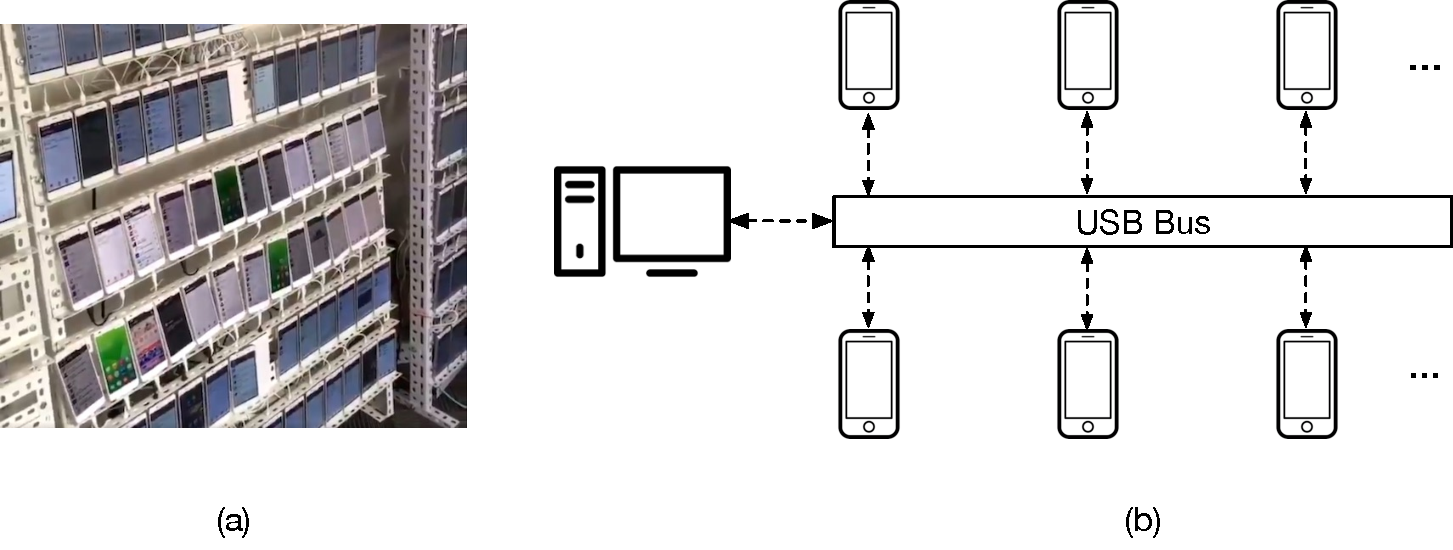
\includegraphics[width=0.44\textwidth]{Figures/clickfarm}
	\caption{(a) A photo inside a real-life click farm \cite{clickphoto}. (b) The general set up of a click farm, where phones are powered up and connected to a central server via USB connections. }
	\label{fig:clickfarm}
	\end{center}
	\end{figure}
	However, despite the effectiveness, 
	setting up such a farm incurs a substantial cost. The major expenses is for purchasing the massive number of devices. Meanwhile, the subsequent deployment and maintenance tasks also involve huge labor costs.
	These drawbacks naturally inspire us to investigate the potential of replacing the physical devices with device emulators. Device emulators are in essence virtual machines that are mainly designed for developers to swiftly prototype mobile applications without using hardware devices. Compared with physical devices, emulators are significantly more cost-effective because they can be massively deployed in cloud platforms or local servers in a cheap price. For instance, the average price for a low-end smartphone with one-year lifespan is approximately 215 USD \cite{pricesmartphone}, while the money can enable us to host 6 emulator instances without optimization in the cloud for a same timespan \cite{vpscom}. Besides, deploying and maintaining emulators is less labor intensive owning to existing automated management systems \cite{mutti2015baredroid}.

	Though the idea of launching click fraud with emulators seems quite straightforward, practical implementation entails substantial challenges. 
	First, existing device emulators are CPU-intensive and memory-intensive. It likely results in poor performance and application failure due to resource constraints. Moreover, the high resource demand also decreases the number of emulator instances that can be run concurrently, which limits the power of the attack. % Meanwhile, it inevitably  . 
	% In other words, it reduces the scale of an attack with a limited budget. 
	Second, the existing emulators are easily blocked by various mobile applications due to their defective device profiles. A profile serves as a unique device signature, usually consisting of properties such as WiFi MAC addresses or phone numbers that are hardware-specific. Since the corresponding hardware components are not emulated, the property values remain empty. Therefore, by scrutinizing the defective device profile, an application can easily identify and block the emulator.
	% each mobile application account, in order to remain active, is required to associate with a unique hardware-related device profile.
	Finally, it is challenging to deploy and manage numerous emulator instances in a large-scale attack, because existing emulator management systems are centralized and they fail to cope with the scale-out and fault tolerance issues. 

	 
	% The high resource usage greatly decreases the number of emulator instances that can be run concurrently given certain cloud resources. 
	% Specifically, existing emulators are mainly designed for developers to swiftly prototype and test Android applications without using hardware devices. 
	% They lack several important features required by a successful large-scale attack.

	% First, the emulators only provide limited or even no emulation for some hardware components of a real device (e.g., a cellular modem). It renders some important functionalities such as receiving text messages and dialing a phone call unusable in an emulator. However,  these functionalities are indispensable when launching attacks on a great number of mobile applications guarded by text message verification. It require a device to have a genuine phone number and be able to receive text messages for verification codes before certain actions are granted (e.g., registration or posting). 


	In this paper, we propose Fraus, a novel approach that enables individuals to launch MCFA using device emulators. Specifically, Fraus significantly reduces CPU usage by circumventing the compute-intensive graphics emulation. It also maintains a small memory footprint by applying the lazy-loading and deduplication techniques on system components. To bypass device-profile scrutiny, Fraus implements two virtual hardware components including cellar modems and WiFi interfaces. They enable each emulator instance to generate a seemingly authentic device profile. Meanwhile, Fraus offers a distributed emulator cluster management system, which is scalable, fault-tolerant and easy-to-use. Its API abstraction features a logically centralized view, which allows an user to easily program and launch an attack task without concerning the details of the underlying distributed protocols.
	% A memory isolation mechanism is also introduced to allow multiple applications to run on a same instance 

	We consolidate the above techniques and implement the prototype of Fraus on top of Android 6.0. We conduct comprehensive experiments to evaluate Fraus against the top 300 applications from the Google Play store. Experimental results show that Fraus has high application compatibility and system stability because 96\% of the selected applications run successfully, while the number is only 59\% for existing emulators. Fraus also reduces CPU usage and memory footprint up to 90\% and 60\% respectively compared with the existing emulators. The small resource demand enables fitting 125 instances in a low-end server equipped with 32GB RAM, reflecting the high cost efficiency.
	% All the applications run smoothly on Fraus, indicating its high system stability. A cluster consisting 500 virtual devices is also set up to demonstrate the Fraus's scalability.
	% \textbf{Rephrase it! And add countermeasure, make it politically correct.}

	To the best of our knowledge, Fraus is the first system that is designed to launch a cost-efficient and scalable MCFA via devices emulators. By designing Fraus, we aim to raise public concerns about the simplicity of committing click fraud and to suggest countermeasures to mitigate such risks.

	% The main contributions of this paper are as follows:
	% \begin{enumerate}
	% \item We present approaches to circumvent CPU-intensive display emulation and to reduce memory usage without affecting system stability.
	% \item We implement a set of virtual devices and drivers that enable an emulator to generate a unique device profile. \textbf{Rephrase it ! And add countermeasure}
	% \item We conduct experiments to confirm the high performance and scalability of our prototype. 
	% \end{enumerate}

	 % Specifically, to bypass text message verification, Fraus utilizes a custom-tailored Android emulator, which emulates the text-messaging and phone dialing functionalities with the help of on-line virtual phone services.  Besides, to keep a tiny memory footprint (around 130 Mb), Fraus carefully prunes a great number of non-essential Android system services while making sure the system stability in not affected. Fraus only requires a small CPU processing power as it avoids the most compute-intensive emulation of video display and audio playback. Meanwhile, Fraus also utilizes a elastically scalable network architecture that automatically deploys and manages the emulator instances in popular cloud services.  

	% The emulator instances along with the automation scripts then will be automatically deployed to popular cloud services 

	% After composing the automation scripts, the emulators will be automatically deployed in a elastically scalable network architecture residing in remote cloud. 

	% We should talk about some experiments?

	The rest of this paper is organized as follows. Section.~\ref{motivate} investigates the problems of launching MCFA using existing emulators.
	% Section.~\ref{overview1} overviews the architecture design and the key components of Fraus.
	Section.~\ref{Circuvment} presents the approach to disable the compute-intensive graphics emulation. Section.~\ref{memory} describes optimization techniques that reduce the memory footprint. Section.~\ref{deviceid} illustrates the methodology to bypass device profile scrutiny. Section.~\ref{deploymentarch} elaborates the architecture for the distributed emulator instance management system.  Section.~\ref{expm} reports the evaluation results. Section.~\ref{countermeasure} discusses the countermeasures to combat Fraus. Section.~\ref{related} surveys the related work and Section.~\ref{conclusion} concludes this paper.


	\section{Background and Motivation}\label{motivate}
	Little research has been conducted to investigate the usability of emulators on MCFA. 
	In this section, we attempt to evaluate the usability and identify the potential problems pending to be addressed via preliminary experiments.
	% In this section, we conduct some preliminary studies by 
	% A click fraud attack can be roughly separated into two essential stages; the first step is to register a scam account and the second step is to repeatedly generate click events with the account. Take Facebook as an example, the malicious will by all means register a huge number of the application accounts and automate them to generate phoney 'likes' by clicking the 'thumb' button. 
	We first select 4 target mobile applications from two genres that are frequent victims of MCFA, including social media and online advertising. The selected social media applications consist of \textit{Facebook} and \textit{Wechat}. The selected online advertising applications, which reward users for every view of a commercial video clip, include \textit{Daily Cash} and \textit{Lucky Cash}.
	We run these applications on three widely-used options including \textit{Android Official Emulator} \cite{andemu}, \textit{BlueStacks} \cite{bluestack} and \textit{GenyMotion} \cite{genymotion}. These emulators are allocated with an one-core 2.2 GHz virtual CPU, 512 MB RAM, and 12 MB video RAM with GPU acceleration disabled. This resource configuration is chosen to be close to the specification of a low-end virtual machine provided by most cloud platforms \cite{vpscom}. In our mocking attack, we identify the following difficulties.

	\textbf{Performance Issues.} The first difficulty arises from the performance issues of emulators. We observe that the emulators tend to be CPU-intensive. 
	To demonstrate our observation, we measure the average system-wide CPU usage when the emulators are automated to perform predefined tasks such as clicking a like button or viewing a video clip in the 4 applications. The results are shown in Table~\ref{tab:precpu}. It can be seen that 
	all the applications are incurring high CPU workload regardless of the types of emulators. Specifically, the social media applications consume almost half of the CPU processing power. The advertising applications appear to be more compute-intensive and nearly saturate the CPU. 

	To pinpoint the root cause of high system-wide CPU utilization, we further demonstrate the usage of each running process in an emulator in Table~\ref{processcpu}. Note that we only list the CPU statistics for the Android official emulator because different emulators yield similar CPU performance. One essential finding from the table is that although the overall CPU usage is high, only a small proportion is attributed to the application itself. Two system processes \textit{Surfaceflinger} and \textit{Mediaserver} are the main culprits of the excessive CPU usage. Surfaceflinger is an Android system service, in charge of compositing graphical user interfaces (GUI) of applications into a single buffer, which is finally displayed by a screen. Mediaserver is another important system service that entitles an application to play various types of video files. The two system services involve a great amount of graphical computation, which can be offloaded to GPUs in physical devices. However, GPUs are not available in an emulator and the graphical computation has to be conducted by CPUs inefficiently,  which justifies the high CPU workload of the Surfaceflinger and Mediaserver.

	% The two system services are the core components of the Android graphics system. In a physical device,  

	%
	% the CPU consumption does not significant differ regardless of the emulators being used. Therefore, it allows us to conduct the remaining analysis on just one type of emulator.

	\begin{table}[t]
	\centering
	\footnotesize
	\caption{System Wide CPU Usage When Running Selected Applications.}
	\label{tab:precpu}
	\setlength\tabcolsep{10pt}
	\begin{tabular}{|l|l|l|l|}
	\hline
	CPU Usage  & Offical & BlueStack & GenyMotion \\ \hline
	Wechat     & 43\%    & 47\%      & 45\%       \\ \hline
	Facebook   & 57\%    & 54\%      & 59\%       \\ \hline
	Daily Cash & 79\%    & 76\%      & 78\%       \\ \hline
	Lucky Cash & 87\%    & 83\%      & 84\%       \\ \hline
	\end{tabular}
	\vspace{-0.2in}
	\end{table}
	% \begin{figure}[ht]
	% \begin{center}
	% 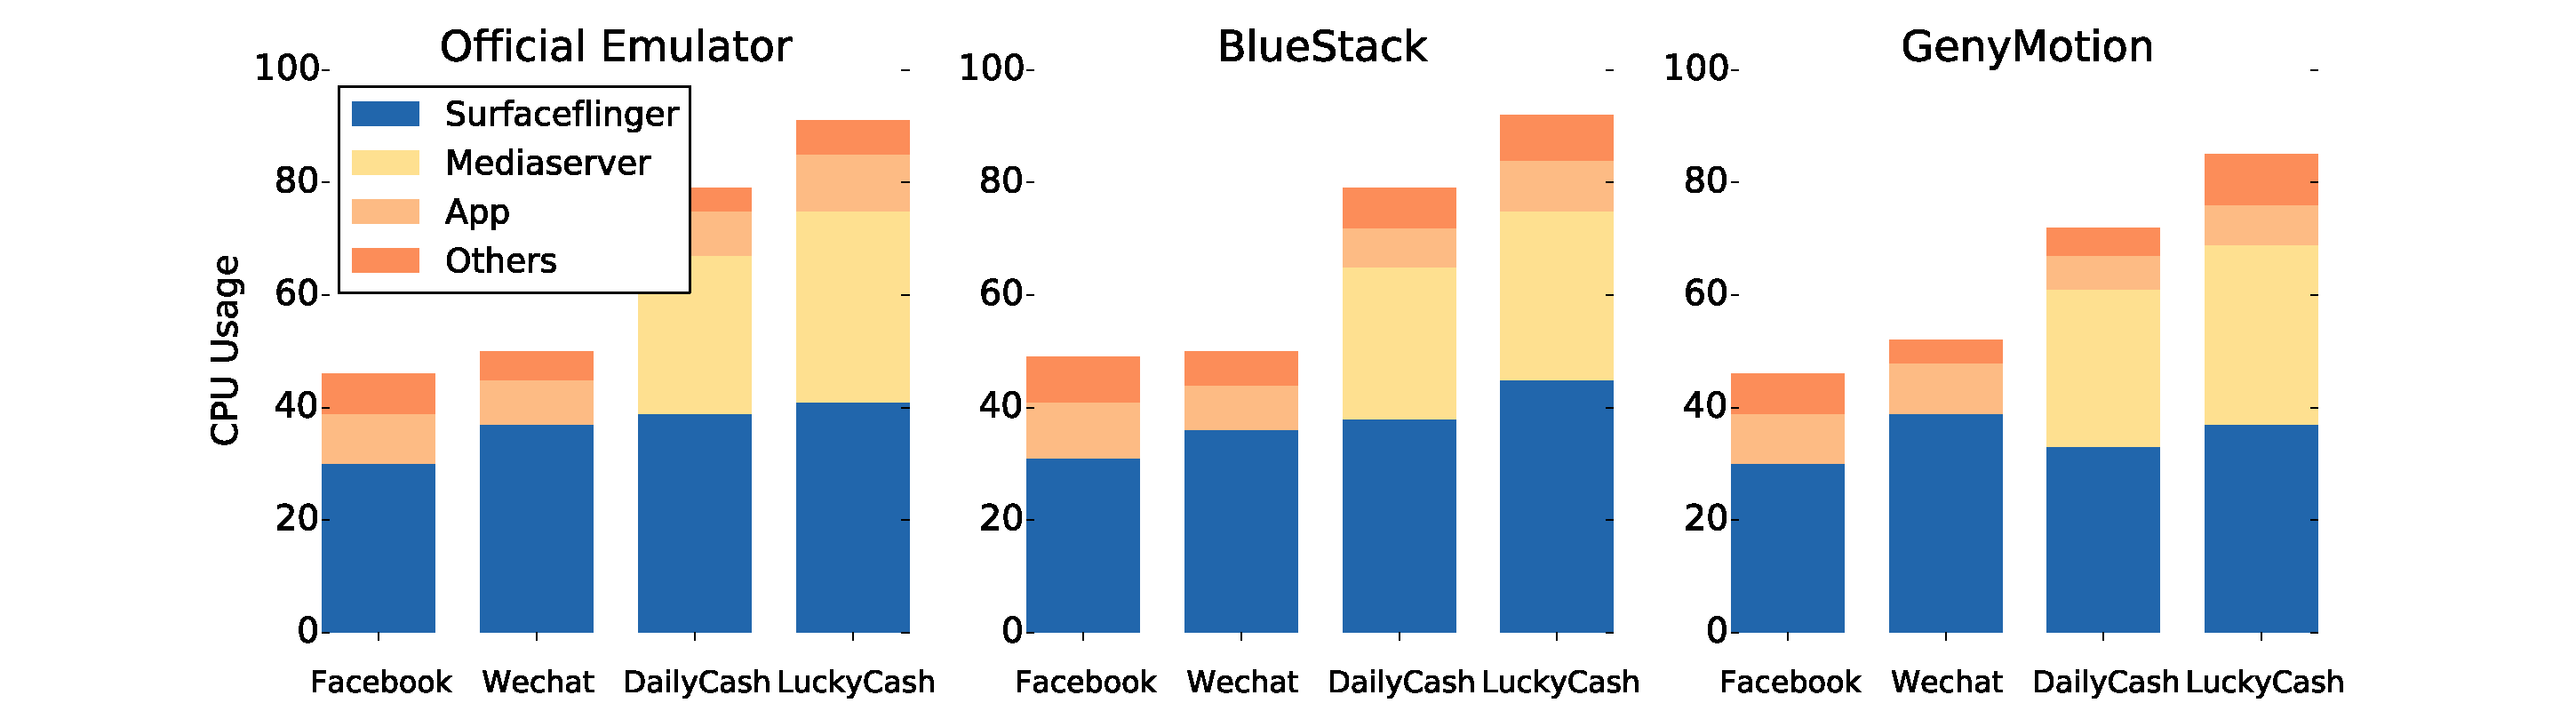
\includegraphics[width=0.50\textwidth]{Figures/precpu}
	% \caption{Typical system deployment.}
	% \label{fig:precpu}
	% \end{center}
	% \end{figure}

		
		\begin{table}[t]
		\footnotesize
		\centering
		\caption{CPU utilization of each running process in an emulator.}
		\label{processcpu}
		\setlength\tabcolsep{0.4pt}
		\begin{tabular}{|l|l|l|l|l|l|}
		\hline
		CPU Usage  & Surfaceflinger & Mediaserver & Systemservice & App. itself & Others \\ \hline
		Wechat     & 25\%           & 0\%         & 3\%           & 11\%        & 4\%    \\ \hline
		Facebook   & 37\%           & 2\%         & 4\%           & 13\%        & 1\%    \\ \hline
		Daily Cash & 11\%           & 49\%        & 7\%           & 7\%         & 5\%    \\ \hline
		Lucky Cash & 23\%           & 43\%        & 5\%           & 10\%        & 6\%    \\ \hline
		
		\end{tabular}
		\vspace{-0.1in}
		\end{table}
			
	%  and it can be
	% seen that regarding the official Android emulator, it occupies full CPU power regardless of the applications are running. Even that, the running applications are still suffering from noticeable lag. On the other hand, the GenyMotion emulator consumes significantly less CPU power when executing social media applications. However, advertisement applications still exhaust a huge portion of CPU capacity.

	Another performance concern is the excessive memory usage. The minimum memory requirement of BlueStack and GenyMotion is 2 GB. It means that the only way to run them in the virtual machine with 512 MB RAM is to enable swapping. However, swapping may negatively impact the system performance due to the potential thrashing behavior. The Android official emulator somehow possesses a smaller footprint, which is approximately 500 MBs right after the system starts up. Nevertheless, the free RAM is extremely limited and swapping is still required in order to run any other applications. 
	 % We examine the memory statistics by using the \textbf{PS} command. We notice that a process name \textbf{system\_server} consumes a huge amount of memory (around 127 MB) 

	% It is clear to see that given certain computational resources, the extensive CPU usage and memory footprint could greatly reduce the number of emulators that can be run concurrently. It then limits the scale of the attack that an attacker can carry out. 

	\textbf{Defective Device Profile.} We meet the second obstacle when running applications that enforce device profile scrutiny. A device profile serves as a unique device identification. It usually consists of several hardware-specific properties. Commonly used properties include:
	\begin{enumerate}
	\item WiFi Media Access Control (MAC) Address, a unique identifier assigned to WiFi interfaces.
	\item The cell phone number of the device.
	\item International Mobile Subscriber Identity (IMSI), a unique number to identify the user of a cellular network.
	\item International Mobile Equipment Identity (IMEI), a unique 15-digit serial number given to every mobile phone's cellular modem.
	\end{enumerate}
	All the properties are retrieved from hardware components including cellular modems and WiFi interfaces. Since they are not emulated,  the above property values remain empty in an emulator. The artifact then allows application providers to easily identify and block the emulators. To make matters worse, the authenticity of the properties, especially the phone number, can be easily verified by the applications. For instance, many applications send the number a SMS containing verification codes to ensure the number is genuine. It makes randomly generating the property values an infeasible approach to bypass the scrutiny.


	% only regard a view as an authenticated one when the device's profile is currently associated with one account. Since all emulators share one dummy profile, if we sign in various accounts in different emulators, we could easily breach the criteria.
	% To defeat scam accounts, all the mobile applications we are testing have implemented text-message verification. It requires a user to have a genuine phone number and be able to receive text messages for verification codes before the registration can be finished. However, the existing emulators only provide limited or even no emulation for the cellular network modem, rendering the indispensable functionalities such as receiving text messages and dialing a phone call unusable. In other words, the existing emulators are not able to bypass the text-message verification.

	% We also notice that some applications further adopt Device-ID verification to prevent attackers from registering scam accounts. During the registration process, the applications will note down some device-specific information. Usually, it contains Media Access Control (MAC) addresses of bluetooth and WiFI interfaces. The information is theoretically unique for every smart device and can be used as a device-id. The device-id verification  will usually enforce every newly registered-account should be associated with a never-seen device-id.  Therefore, the emulators are not able to bypass the Device-ID verification.

	\textbf{Deployment and Management.} 
	We encounter another challenging issue when launching a large-scale MCFA. In such an attack, a massive number of emulator instances have to be deployed and managed. To avoid this labor-tensive procedure,
	% Clearly, it would be labor-consuming and error-prone to set up and monitor all the instances manually. We require a device management system that can automate this procedure. 
	we adopt a centralized cluster management system \cite{mutti2015baredroid} in our preliminary study. However, we discover that the centralized architecture quickly fails to cope with the scale-out and fault tolerance issues when the number of emulators dramatically increases. To address this issue, we need to design a distributed management system. Meanwhile, to preserve the simplicity of the centralized management system, we aim to design a high-level API abstraction presenting a logically centralized view, which can conceal the complicated details of the underlying distributed protocols. 

	% How to design the architecture remains a challenging issue. 	

	In light of the above issues, we design Fraus, a system that is lightweight and able to bypass the device profile scrutiny. Meanwhile, Fraus's distributed emulator management system enables us to launch a large-scale MCFA in an effortless manner. In the following sections, we will elaborate Fraus's solutions towards the above issues one by one.



	% it is effortless to launch a large-scale click fraud attack with the help of . 


	% it is necessary to design The API interfaces should ensure 




	% When designing a distributed architecture, we aim to maintain 

	% Second, to monitor and control the huge number of devices, it may be inappropriate to adopt a simple centralized architecture since it fails to cope with the scale-out and fault tolerance issue when the number of virtual devices increases. In other words, a more sophisticated distributed architecture to  is required. 




	% The whole process can be mainly divided into two phases. In the first stage, the scheduler submits (testing/probing/?) Packet-in requests to controllers in an arrival rate growing exponentially. It begins with an initialized arrival rate $r_{init}$ (e.g., $r_{init}$=1000 pkts/s) and increases by one when a \textit{Packet-Out} response is received. The intuition is that the response time of controllers under relatively low workload barely varies. An exponential growing rate helps accelerate the process.
	% The first phase is called \textbf{Fast Start}, in which the \textit{Packet-In} arrival rate $r$ grows exponentially in order to accelerate the whole process. In details, it begins with an initialized arrival rate $r_{init}$ (e.g., $r_{init}$=1000 pkts/s) which will increase by one packet for each \textit{Packet-Out} returned. Simultaneously, the corresponding packet processing time $t$ and CPU utilization $u$ are recorded. As $r$ increases, the workload of the controller grows as well. There exists a certain point that the high workload of the controller leads to dramatical increase of $t$. Specifically, the dramatic grow of $t$ is detected when its value is more than two standard deviations from its mean value. At that time, the process enters its second phase called \textbf{Overload Avoidance}. In this phase, $r$ will be first decreased (e.g., reduce to ${3/4}$ of its current value) to avoid controller being overloaded. Until the dramatic grow disappears, the growth of $r$ will be slowed down to linear increase (e.g., 1000 pkts/s) until next dramatic increase of $t$. This process repeated until the difference between two consecutive CPU utilization $u$ less than a predefined threshold (e.g., $0.1$). Then the CPU utilization $u$ is the threshold $H$.



	\section{Preserving CPU Resources}\label{Circuvment}
	As stated in the previous section, due to the lack of GPUs in an emulator, graphical computation such as GUI composition and video playback has to be conducted by CPUs inefficiently, which results in a huge waste of CPU resources. In this section, we elaborate our approaches to preserve the CPU resources for an emulator. The main intuition is that we can circumvent the graphical computation in Android because attackers most of the time do not care about the graphical output of the emulators, which are running automation scripts to generate click events.

	\subsection{Overview of the Android Graphics System}
	To make our approaches better understood, we first introduce the architecture of the Android graphics system. As shown in Fig~\ref{fig:graphics}, an Android application can draw its contents on the device screen via three different routines including \textit{Skia}, \textit{OpenGL} and \textit{Media Server}.

	\begin{figure}[t]
	\centering 
	\captionsetup{justification=centering}
	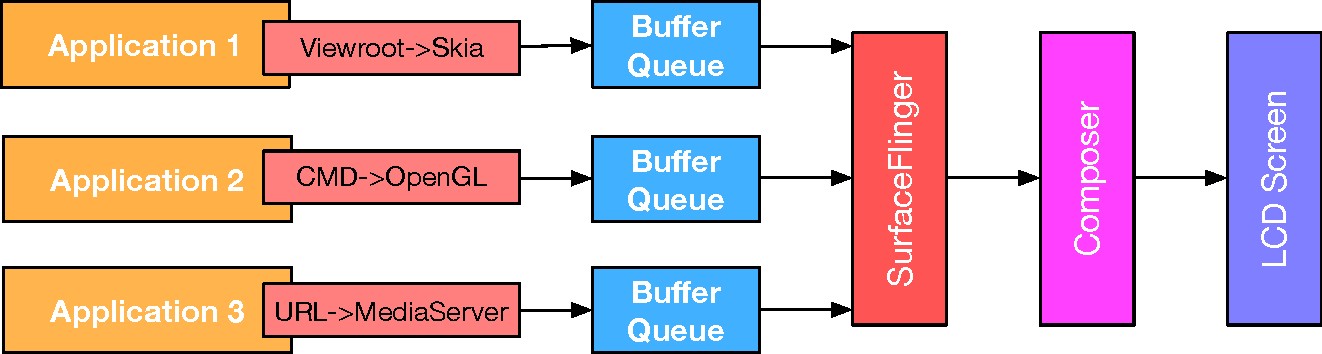
\includegraphics[width=0.45\textwidth]{Figures/graphics}

	\caption{Android Graphics Overview}
	\vspace{-0.3in}
	\label{fig:graphics}
	\end{figure}

	\textbf{Skia.} The most commonly-used routine relies on the \textit{Skia} library to performs 2D graphics drawing. Specifically, an application provides the Skia with its GUI layout hierarchy, which organizes all the GUI components (such as texts, buttons and images) in a tree structure. The tree's root is referred to as \textit{ViewRoot}. Beginning with the ViewRoot, drawing is performed by walking the tree and rendering all child components by invoking their \textit{draw()} method. The method draws the GUI component's appearance on top of a graphics buffer. The resulting buffer then can be inserted into a buffer queue and wait for the further processing from the underlying system service.

	\textbf{OpenGL.} An application can perform 3D graphics drawing with the help of the \textit{OpenGL ES} library. OpenGL ES is a cross-platform graphics API set that specifies a standard interface for GPUs. By invoking the APIs, applications could deliver 3D drawing commands to GPUs. Once GPUs finish the tasks, the resulting buffers will be also inserted to a buffer queue. Note that emulators possess no GPUs, thus they have to be emulated via software.

	\textbf{Media Server.} An application can utilize a system service named Mediaserver to display video contents on the screen. Specifically, the media server accepts a media file and processes it by using built-in media decoders. The decoded buffers then will be sent to the buffer queue. Note that the video decoding is considered to be a fairly CPU-intensive procedure, a physical device therefore usually offloads it to the a dedicated hardware decoder that does not exist in an emulator. 
	 
	All the routines places the resulting buffers to the buffer queues. The queues are managed by a system service named Surfaceflinger. Specifically, Surfaceflinger will dequeue the buffers from all the queues and forward them to the underlying composer. The composer then composites all the buffers and generates a final picture on the screen. The process is carried out periodically and the frequency is decided by the LCD screen hardware. In brief, the hardware will indicate the Surfaceflinger to start the process by generating a VSYNC signal. In an emulator, the VSYNC signal is generated from a software timer every 1/60 second. 

	\subsection{Naive Approach: Suppressing VSYNC Signal}
	A simple solution to skip the graphical computation is to suppress the VSYNC signal by adjusting the software timer. Without the VSYNC signal, the Surfaceflinger would stop dequeuing buffers from the buffer queues. Then the number of buffers in the queues would start accumulating. Once the number reaches a limit, which is three by default, the Android applications would not be able to enqueue more graphics buffers and have to stall the drawing process. In order words, no more draw() methods would be invoked and the graphical computation would be circumvented.

	Despite the simplicity of the approach, it may affect the stability of certain applications that contain custom GUI components. Custom components entitle developers to create novel user interfaces for special needs. To implement such a component, developers have to write their own draw() method and manipulate the graphics buffers to sketch the component's appearance. Besides, auxiliary functionalities such as performance tuning and logging may also be implemented in the draw() method. Since the draw() method is suppressed by our approach, the auxiliary functionalities would never get the chance to be executed, which may potentially crash the applications.




	% contain custom GUI components. Custom components entitle developers to create novel user interfaces for special needs. To implement such a component, developers have to write their own draw() method and manipulate the graphics buffers to sketch the component's appearance. Most of the time, developers also implement other  in the draw method(). For instance, some applications keep the track of frame rates and use them as a indicator whether the application is running normally. 

	% In details, Android allows developers to create custom GUI components for special needs not covered by the built-in components. 


	% have overwritten the draw() method. Android allows developers to overwrite the draw() method such that they can create custom GUI components for special needs. 

	 % It may disrupt the applications with custom GUI components. . To implement a custom components, developers have to override the draw() method and draw graphics primitives using Skia or OpenGL. However some applications also insert other procedures such as performance tuning and logging in the method. Thus, those procedures may be seriously disrupted because the drawing process is suppressed and no \textit{draw} method is invoked. It likely leads to the instability of the application.

	 % athe screen hardware will generate a VSYNC signal every 1/60 second, which serves as a timer to trigger the process. 

	% In other words, every 1/60 second passes, the display system will generate a traverse event to re-initiate the drawing process.
	 % SurfaceFlinger knows the layout of all the UI windows in the system by working with the WindowManager service. Smartphone displays typically re- fresh at a rate of 60 fps and for each frame period the system generates a VSYNC signal. When a VSYNC signal arrives, SurfaceFlinger collects all the graphics buffers for visible lay- ers and asks the Hardware Composer to composite all visible layers together. Usually the Hardware Composer will do the composition itself and generates the final graphics data into the system Framebuffer for displaying on the screen. Some- times the Hardware Composer may determine that the most efficient way to composite the buffers is using the GPU and thus asks SurfaceFlinger to call OpenGL ES API to use the GPU for buffer composition. In this case, SurfaceFlinger also generates GPU workload. After SurfaceFlinger consumes a graphics buffer in a BufferQueue, the corresponding appli- cation is notified for drawing a new frame.

	% accepts a buffer assigned by the display system and draws the appearance on top of it using low-level graphics APIs.
	% {}
	% On Android, OpenGL ES/EGL1 is used for GPU-accelerated graphics. Applica- tions call the OpenGL ES API [31] to use the GPU for graph- ics processing and to draw their User Interface (UI). The processing result is put into a graphics buffer in a structure called BufferQueue. Each application has its own Buffer- Queue that has three graphics buffers by default. The sys- tem UI process also has a dedicated BufferQueue for drawing the system UI elements such as the “navigation bar” at the bottom of the screen and the “status bar” at the top of the screen. Android uses a system service called SurfaceFlinger to co- ordinate all the graphics layers from the running applications and the system UI process. SurfaceFlinger knows the layout of all the UI windows in the system by working with the WindowManager service. Smartphone displays typically re- fresh at a rate of 60 fps and for each frame period the system generates a VSYNC signal. When a VSYNC signal arrives, SurfaceFlinger collects all the graphics buffers for visible lay- ers and asks the Hardware Composer to composite all visible layers together. Usually the Hardware Composer will do the composition itself and generates the final graphics data into the system Framebuffer for displaying on the screen. Some- times the Hardware Composer may determine that the most efficient way to composite the buffers is using the GPU and thus asks SurfaceFlinger to call OpenGL ES API to use the GPU for buffer composition. In this case, SurfaceFlinger also generates GPU workload. After SurfaceFlinger consumes a graphics buffer in a BufferQueue, the corresponding appli- cation is notified for drawing a new frame.



	\subsection{Sophisticated Approach: Submitting Blank Buffers}
	Clearly, the main drawback of the naive approach is that it may interfere with the application execution and the final outcome varies from application to application. Motivated by this issue, we propose a more sophisticated approach that is more reliable and fully application-independent. The main idea is that we alter the behavior of the three graphics routines; they now simply submit blank buffers to the buffer queues, when applications request them to draw any contents. This approach not only circumvents the intensive graphical computation, but also poses no interference to all applications. From the applications' viewpoint, they can invoke the draw() method periodically as they are running in a normal Android system.




	% the three graphics routines spend enormous CPU resources to generate correct graphics buffers, while the correctness is unnecessary. Thus, our approach alters the behavior of the routines such that they simply submit empty buffers to the buffer queues.

	% to skip the computation.

	%  For instance, when an application decides to draw a line, the Skia library has to conduct complicated geometry calculation such that the line can appear in the correct position on the screen. In our approach we replace the complicated calculation, 


	% Since the screen content is not used by the attackers, 
	% As we state before, the graphical output of applications is . Therefore, the correctness of the results of graphical computation are not important.

	% the high CPU is generated when executing the graphical computation codes insides the three routing.  that the correctness of the resulting buffers from the Skia, OpenGL and Media Server does not matter and we could directly submit an blank buffer to the queue and skip the core graphical computation. By this mean, we could preserve a large amount of CPU processing power without disrupting an application's drawing process. 

	% One straightforward way to achieve this is to modify the corresponding source codes of the Android framework. However, the method cannot be applied generally to different versions of Android, which keeps updating its source codes in a staggering pace. Instead, 

	We implement this approach by adopting a technique named Dynamic Linker Hooking \cite{hooking}.
	Specifically, hooking is the process of intercepting a program's execution at a specific point, typically entries of functions, in order to alter or augment the program's behavior. The dynamic linker hooking technique enables hooking in the runtime by forcing a program to load shared libraries specified by the user instead of the original ones provided by operating systems. This technique allows us to avoid recompiling the source codes of Android and to quickly apply the following patches to the three graphics routines.
	% only need to patch a small number of functions as follows.

	\textbf{Skia.} 
	We patch all the low-level Skia APIs to avoid the drawing procedures. Specifically, Android internally draws each GUI components by invoking a series of low-level Skia APIs such as \textit{SkBitmapDevice::drawPaint}, \textit{SkBitmapDevice::drawPoints}, and \textit{SkBitmapDevice::drawRect}. The APIs originally conduct compute-intensive linear algebra computation to place correct shapes on a graphics buffer. After the patching, these APIs become stub functions which simply return a result indicating the rendering operation has been successful. 

	% Considering that the correctly displaying shapes is not necessary in our case, our approach replaces each function with a stub one skipping the heavy CPU computation.  to the display system and each drawing process can still be carried out without incurring heavy CPU usage. 
	\textbf{OpenGL ES.}
	The stock OpenGL ES library only supports a very basic set of OpenGL commands and it is barely compatible with modern Android applications \cite{zechner2016android}. To address this issue, 
	we first replace the stock OpenGL ES library with a fully-fledge open-source one \cite{graphics2008mesa3d}.
	Two kinds of patches are then applied on the library. First, we rewrite all the graphics APIs whose names start with \textit{glDraw}. The modified functions skip the complicated 3D geometry rendering and simply report a result indicating operations are successful. 
	Second, we also patch the \textit{memcpy} function used in the graphics APIs including \textit{glBufferData} and \textit{glCopyTexImage2D}. The two APIs are originally designed to copy bulky texture data from the user process to the GPU emulator. Realizing the excessive data transfer may negatively degrade system performance, we replace the \textit{memcpy} function with a no-operation (NOP) to skip the data copying.

	\textbf{Media Server.}
	% The system service Media Server handles the playback of the video file in an Android application.
	% Apart from rendering views, another important functionality provided by the display system is video and audio playback. 
	% Android provides a multimedia framework that allows developers to integrate video and audio files in the apps.
	We patch the commonly-used media decoders including \textit{mpeg2dec}, \textit{avcdec} and \textit{aacdec} in the media server. As shown in Fig.~\ref{fig:mediaserver} (a), the origin decoders repeatedly request a media access unit from the source. The unit then can be decoded into a displayable frame or a few milliseconds audio clip, which will be sent to a buffer queue. The playback is finished if the decoders successfully detect the end of stream (EOF) in the source. 

	To avoid decoding computation, we let the decoders dump the access units received and directly send frames filled with zero to the buffer queue. However, this method has a limitation; without running the decoding algorithm, the decoder now cannot determine how many audio frames exist in an audio access unit. If the decoder cannot generate a correct number of audio frames, the duration of the playback may be either shortened or prolonged. It may affect the stability of certain applications, for instance, advertisement applications which rely on the duration of playback to count a view. 

	To address this issue, we propose an alternative solution  as shown in Fig.~\ref{fig:mediaserver} (b). The patched decoder will infer the number of frames needed to be generated by examining the timestamp property existed in access units. Specifically, every access unit carries a timestamp indicating the time at which its first decoded frame is played. The timestamp difference between the current and consecutive access units then can be used to calculate the available frames given the audio sampling rate. 

	\begin{figure}[tb]
	\begin{center}
	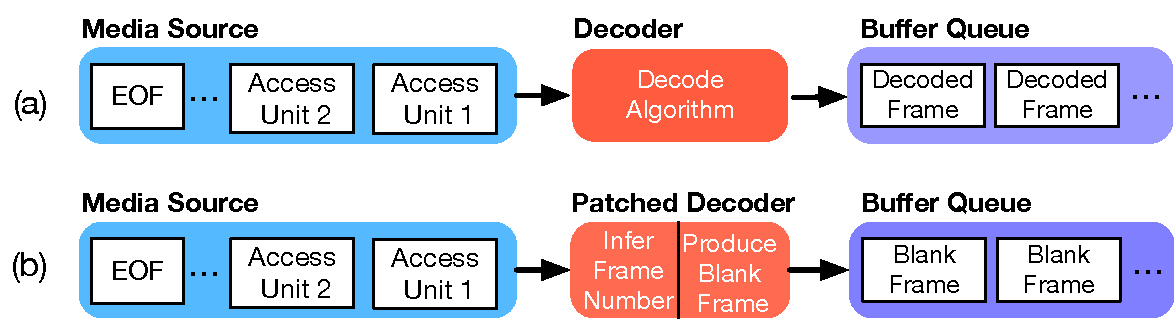
\includegraphics[width=0.44\textwidth]{Figures/mediaserver}
	\caption{(a) The decoding process of the media server. (b) The patched decoder avoiding the decoding computation.}
	\label{fig:mediaserver}
	\vspace{-0.3in}
	\end{center}
	\end{figure}


	% \textbf{Disabling Audio System}
	% The Android audio system also drains a significant amount of CPU capacity. The audio system receives audio streams from multiple apps and perform audio post-processing including filtering noises, applying audio effects, and mixing before the final playback. In details, the system service AudioFlinger maintains a ring buffer for each app. Applications put the audio data in the buffer and the AudioFlinger will consume and process it with the help of a thread named MixerThread. In our system, we extend the MixerThread and override the threadLoop() method such that the thread just periodically removes the data in the ring buffer to skip the audio processing.

	% The existing emulators tend to consume intense CPU and memory resources.
	% We first investigate the cause with the help of performance profiling tools provided by Google \cite{}. The tools enable developers to record an app's compute, memory and rendering performance, which provides immediate insight to the performance issues.

	% \subsection{Reducing CPU Usage}
	% We now turn our focus on the CPU usage optimization. The preliminary experiments in Section shows that the official Android emulator occupies full CPU power regardless of the apps are running. On the other hand, the Genymotion consumes moderate CPU while running social media apps, though the advertisement apps still exhaust a huge amount of CPU capacity. 

	% To better understand the performance gap between the two emulators, we apply the CPU profiling tool on the two emulators run identical apps. The apps are instructed to perform a set of predefined tasks. Meanwhile, the profiling tool will enable method tracing, which entitles us to log the call stack and timing information of each method for the apps. By this means, we could compare the CPU time elapsed for a same procedure on the two emulators. We observe that the CPU time consumed by the official Android emulator is at least 5 times longer than that used by the Genymontion. After an in-depth investigation, we discover that the performance gap is mainly owning to the CPU instruction each emulator is emulating. More specifically, the official Android emulator is featuring an ARM emulation architecture, while the Genymotion is using x86 architecture virtualization. Note that emulating ARM instructions on a x86-64 host is rather CPU intensive as it requires dynamic binary translation from ARM to x86. On the other hand, emulating x86 instructions on a modern computer is mostly effortless due to hardware assisted virtualization technology [], which explains the performance gain of the Genymotion.

	% We also investigate the cause of another important phenomenon that advertisement apps are more CPU-intensive than social media apps. By sorting and comparing the trace data of the two types of apps, we notice that the advertisement apps spend mass CPU time (approximately 90\%) on display system while the number for social media apps are significantly lower (about 27\%).
	% This matches the intuition that the advertisement apps are designed to showcase all kinds of commercial clips and update  display frequently; conversely, the social media apps tend to be more static in terms of screen contents. It can be seen that the heavy load on the display system is a major factor that leads to extensive CPU usage.

	% Motivated by the two observations, we propose two optimization approaches to reduce the CPU usage.

	% \textbf{Applying X86 Architecture.} Fraus compile the Android system from source for x86 platforms. By doing this, the emulator can avoid the excessive overhead of ARM instruction emulation. 

	% Despite that the idea is straightforward, practically implementing it entails a challenging issue. Specifically, Android supports apps written either in Java or C/C++ languages. Regarding the apps purely written in Java, the underlying CPU architecture is transparent to them as the Java compiler has transformed their source codes to platform-independent byte codes. As for the apps with components written in C/C++, the apps are likely to crash because the C/C++ components have been compiled to ARM instructions, which are incompatible with x86 platforms. Though a small number of apps are shipped with x86 versions, the other apps will not be able to run in the emulator.

	% To address this issue, Fraus adopt a technique introduced in []. The technique allows real-time binary instruction translation from ARM to x86. Note that compared with the official Android emulator, our approach merely translates a small number of components with ARM instructions such that a great amount of overhead is avoided.

	% \textbf{Making Emulator Headless.}
	% From a click fraud attacker's view point, displaying contents on a screen is the least necessary functionality so long as an app could still run properly. This presents us a change to further preserve CPU resources by disabling the heavy-loaded display system. 

	% The Android display system handle the procedure for drawing when an app starts running. In brief, an app provides the display system with its layout hierarchy. The hierarchy organizes all the views (i.e., graphical user interfaces for displaying data and interacting with the user, for instance, buttons, texts, and images) with a tree structure as shown in Figure. Beginning with the root node, drawing is performed by walking the tree and rendering each view by invoking their draw() method. The method accepts a buffer assigned by the display system and draws the appearance on top of it using low-level graphics APIs. Once the walking process is finished, all the buffers will be gathered by the display system and rendered in the LCD screen. The whole drawing process is carried out repeatedly at a certain interval. The interval is mainly decided by the refresh rate of the LCD sc]\reen, which is typically 60 Hz. In other words, every 1/60 second passes, the display system will generate a traverse event to re-initiate the drawing process.

	\section{Reduce Memory Footprint}\label{memory}

	In this section, we demonstrate how to optimize the memory footprint of an emulator. The memory-exhausted problem comes from that Android loads nearly all system components to the memory during the booting process, even most of them are not used by applications. In Fraus, we defer the loading of those components until when they are needed. 
	% In this manner, we can save huge amounts of RAM without impeding the system's functionality and stability.
	% The proposed optimization is  based on the official emulator running Android 6.0. The emulator is chosen owning to its relative  memory footprint compared with other options as shown in Section~\ref{motivate}.	

	We first measure the memory usage in the official emulator running Android 6.0. Note that the measurement is conducted right after the booting process and the emulator has been restored its factory settings. 
	The memory statistics shows that the total memory usage is approximately 500 MB, specifically, 290 MB of which is allocated to built-in applications (e.g., calendar, email, and music) while the remaining is consumed by a set of system services (e.g., Systemserver, Surfaceflinger and Mediaserver).

	It can be seen from the statistics that a huge memory overhead lies in the built-in applications, which automatically start along with the system. This behavior is usually referred to as preloading, which helps improve user experience by shortening the applications' loading time. Since these built-in applications are seldom used in a MCFA, preloading them is simply a waste of memory. To reclaim the memory, we patch the applications to disable preloading. Specifically, an application can be preloaded by either registering a listener for the \textit{boot\_completed} event or setting the  \textit{android:persistent} property in its manifest file. Thus our patches remove all the listeners for the boot event and the android:persistent property if existed.

	Apart from the built-in applications, we discover that another major memory consumer are the system services. Android possesses approximately 70 Android system services that provide applications with the information and capabilities necessary to work. 
	Typically, all the services are instantiated by Android during the booting process. However, a great number of them may never be used by an application, which results in the waste of the memory space. 

	% % To address this issue, one straightforward approach is to delete . However, this method possesses a significant drawback. A great number of applications are likely to crash when they attempt to invoke methods provided by the pruned services. Therefore simply removing services may greatly impede the system stability.

	% % To interact with these services, an application relies on a special interprocess communication mechanism named \textit{Binder}. It allows the application to issue a remote procedure call to invoke methods from the system services. For instance, an application can invoke the vibrate() method in the \textit{Vibrator} Service to vibrate a device. 
	% % Although these services are crucial to a physical device, a great of them are likely futile for a device emulator. For example, since there exists neither a battery nor a motor in the emulator, the battery service and vibrator service simply remain idle but still occupy a certain amount of RAM. This offers us an opportunity to reclaim RAM from the System\_server process.



	% % these applications like calendar and music may be seldom used in a MCFA, which leads to a waste of memory.


	%  % every Android applications with the information and capabilities necessary to work.

	% % the RAM resources are mainly occupied by two types of system processes including \textbf {System Services} and \textbf{System Applications}. In details, the process system

	% % \textbf{System Services} 


	% % We examine all the system services and find a great number of them are almost meaningless to an emulator instance. For example, the battery service is in charge of monitoring the health status of a battery. As there exists no battery in an emulator, the battery service simply remains idle but still occupies a certain amount of RAM. Another good example is the vibrator service which manages the vibration motor in a real device. 

	% % One straightforward approach is to remove the unimportant services from the Android framework. However, this method possesses a significant drawback. A great number of applications are likely to crash when they attempt to invoke methods provided by the pruned services. Therefore simply removing services may greatly impede the system stability.

	To reduce the memory footprint, one naive approach is to directly disable certain system services which are unlikely to be used. Clearly, this method may impede the system functionality and stability, because applications are likely to crash when they attempt to communicate with the disabled services. Instead, we propose an alternative approach making use of the lazy-loading and deduplication techniques. Specifically, we first divide all the system services into three categories including  \textit{futile} \textit{occasionally-used}, and \textit{critical} based on the necessity of their functionalities. Then we applied different approaches to reclaim the memory.

	\textbf{Futile Services}
	The futile services such as \textit{Battery Service} and \textit{Vibrator Services} are highly unlikely to be used in an emulator due to the lack of the corresponding hardware components like batteries and vibration motors. However, these services still occupy a certain amount of RAM space due to the memory allocation of internal data structures. To reduce the services' memory overhead, we replace them with stub services. Stub services expose identical API interfaces as the original ones do, but the implementation of the APIs just serves as a placeholder and no memory is allocated. Applications that invoke the APIs will simply receive a result indicating the corresponding operations are successful.

	\textbf{Occasionally-used Services}
	The occasionally-used services such as \textit{MediaRouter} and \textit{TextService} still provide  infrequently-used functionalities to a small number of applications. To reduce their memory overhead, we propose a lazy loading mechanism. It allows these services to postpone the instantiation to when they receive the first request from applications. To implement this mechanism, we first design a set of proxy objects of those services. A proxy object implements same API interfaces as the original services do and forwards the API requests to the corresponding services if they already instantiate. Otherwise, the proxy then is in charge of instantiating the services. Meanwhile, we patch a system process named \textit{SystemServer} such that Android loads the proxy objects instead of the real services to the memory during the booting process. 

	 % and simply forwards to requests to the real services, which are not instantiated 
	% If the desired service is not found, the manager then will set it up. This mechanism greatly avoids the waste of RAM space as occasionally-used services may not be used in most of the time. 

	\textbf{Critical Services}
	The critical services such as \textit{Activity Manager} and \textit{Window Manager} provide the basic system functionalities to every application and thus should remain intact. Nevertheless, realizing these critical services are identical and run in every emulator instance, we can easily infer that in the physical server hosting the emulators, there exists enormous duplication in memory. To reduce the memory usage, we adopt a deduplication technique named Kernel Same-page Merging (KSM). It merges identical memory pages from multiple emulator instances into one memory region, which significantly reduces the memory consumption and increases the number of instances that can be run concurrently.

	% The occasionally-used services will still be registered but remain uninitialized.

	 % An application will contact the manager in order to locate the desired service. If the desired service has been initialized, the manager directly returns the pointer. If not, the service manager could start the initialization.

	% Another huge memory overhead lies in the preloaded system applications.  such as dialer and camera. 

	% Note that the above optimization techniques not only reduce the memory footprint, but also decrease the CPU consumption as well. 

	% They enable users to perform common tasks such as dialing, messaging and photo taking. 


	% The apps can also provide key capabilities to third-party applications. For example, an application could simply invoke the messaging application to deliver a message to the recipient specified. 

	% However, we notice that these apps consume a considerable amount of RAM even an user does not start and use them. We investigate this phenomenon and find that the apps tend to preload themselves to RAM along with the system booting process. It brings an advantage that the starting time of those apps can be reduced for a better user experience. However, since an emulator may seldom use the system apps, preloading them potentially leads to a huge waste of memory. 


	% For instance, the vibrate() method in the original vibrator service contains a series of complicated procedures such as allocating HAL drivers and invoking kernel system calls. Conversely, the method in the stub service simply return a value zero, indicating operation is successful. This approach significantly reduces the memory usage of each service and ensures the apps could still correctly invoke the service methods.

	% \textbf{Content Providers}
	% Just like system services, content providers are also one primary building block of Android applications. A content provider acts like a database managing access to a central repository of data, which is intended to be used by other applications. For instance, the Contact Provider stores the contact information and an app can access the information by inquiring the provider. Another good example is the Media Provider, which contains meta data for all available media on both internal and external storage devices. Therefore, an Album app could list all photos of a user by interacting with the provider. 

	% Content providers inevitable consume certain amounts of RAM for data storage and management. Since most content providers could be considered meaningless for an emulator, we could disable them to gain more memory resources. Thus, Fraus removes all the existing providers and inserts a specially-designed provider to handle inquiries about contact and media information. Though the provider simply returns an empty result to all inquiries, it is still indispensable because numerous Android apps still attempt to access those information for various reasons.  


	\section{Bypassing Device Profile Scrutiny}\label{deviceid}

	As stated in Section~\ref{motivate},
	current emulators are not likely to pass device profile scrutiny, because their device profiles are missing properties including 1) WiFi MAC addresses, 2) IMEI, 3) IMSI, and 4) phone numbers. The main cause of this problem is that the emulators possess no WiFi interface and cellular modem, from which the above properties are retrieved.
	In this section, we demonstrate the approach that bypasses the device profile scrutiny by emulating the missing hardware components. The components help provide a complete device profile and disguise the emulator as a legitimate device. 

	\subsection{Integrating Simulated WiFi Interfaces}
	We first focus on the WiFi MAC address property. A MAC address is an identifier assigned to WiFi interfaces for communications at the data link layer. In a physical device, the MAC address can be accessed by an application using the APIs from the \textit{WiFi} service, for instance, \textit{WifiInfo.getMacAddress()} or \textit{NetworkInterface.getNetworkInterfaces()}. However, in an emulator these methods simply return an empty value or raise an exception complaining of the missing WiFi interface.

	% It may result in the emulator fails to bypass the device profile scrutiny as some applications demand a unique MAC address.
	To address this issue, we enhance the emulator with a simulated WiFi interface.
	In brief, we implement a loadable Linux kernel module that simulates major wireless functionalities and exposes itself as a wireless driver in the same way a common physical WiFi interface does. It maneuvers the Android system and WiFi service into believing that a WiFi interface is properly installed. The simulated WiFi interface then can provide a randomly-generated MAC address. MAC address randomization is widely acceptable \cite{vanhoef2016mac} and it is unlikely that an application will verify the authenticity of the address.
	 % In details, the module exposes itself as a normal wireless driver, which is loaded by the

	\subsection{Emulating Cellular Modems} 
	Compared with MAC addresses, generating legitimate values for the remaining properties (i.e., phone numbers, IMSI and IMEI) is more challenging. These properties are obtained from a cellular network via a modem and they can be easily verified by an application. For instance, an application provider can examine the authenticity of a given phone number by sending it a SMS containing secret codes. The codes are typically required before the user can start using the application. 

	It can be seen that we cannot bypass the scrutiny mechanism by simply generating random property values. Instead, the emulator is required to possess a working phone number and receive SMS from a real cellular network. In Fraus, we achieve this by implementing a software modem that bridges emulators to a cellular network just like a physical modem does. It enables the modem to provide verifiable device profile properties.
	% In Fraus, we implement a software modem that emulates the most essential functionality of a physical modem.

	% that emulates two essential functionalities of a physical cellular modem. First, it provides emulators with the missing device profile properties including phone number, IMEI, and IMSI. Second, it enables emulators to connect to a cellular network and to perform cellular communication (e.g., send/receive SMS). 


	% A cellular modem provides three device profile properties including phone number, IMEI, and IMSI. 
	% Fraus emulates a cellular modem in order to provide device profile properties including phone number, IMEI, and IMSI. Clearly, it is trivial to generate the IMEI and IMSI 

	% A physical device can retrieve device profile properties including phone number, IMEI, and IMSI from a cellular modem. 
	% Without a physical cellular modem, a device emulator is not able to provide cellular network information including phone number, IMEI, and IMSI.
	% The emulated cellular modems should provide two essential functionalities. First, they should provide devices with device profile properties including phone number, IMEI, and IMSI. 

	% they enable Android devices to connect to a cellular network and to perform cellular communication (e.g., send/receive SMS). Second, they can also provide devices with cellular network information including phone number, IMEI, and IMSI. The two functionalities are essential for passing device profile scrutiny. 



	% The emulated modem is integrated into the Android telephony architecture as shown in Figure~\ref{fig:rild}.
	% allow the virtual modem to acquire a mobile phone number programmatically via HTTP connections. The number then can be used to receive in-bound text messages. 

	% Figure~\ref{fig:rild} illustrates how Fraus integrates the emulated modem to the Android telephony architecture.
	% To provide the three device profile properties including IMEI, IMSI and phone number, we integrate a software modem to the Android telephony architecture. 
	To make our approach better understood, we first introduce how the Android telephony system works.
	As shown in Fig~\ref{fig:rild}, 
	% To make our approach better understood, we first introduce the architecture of the Android telephony system. As shown in Fig~\ref{fig:rild},
	Android applications can request the telephony service to perform a set of cellular-related tasks (e.g., sending SMS or dialing numbers) via APIs.  These tasks will be forwarded to a native process named radio interface layer daemon (RILD). The daemon further forwards the requests to the device's modem driver library.
	% The library provides unified interfaces to the RILD regardless of the model of the device's modem.
	The library then translates the requests to modem-recognizable commands (e.g., AT\&T commands) and sends them to the modem for execution. Note that these commands are referred to as solicited commands as they are initiated by the telephony service. Meanwhile, the driver library will continuously monitor the responses of the delivered commands and other radio events (e.g., network ready or new message arrived) that originated from the modem. The responses and events are called unsolicited commands, which will then be propagated to the RILD and upper layers.
	 Note that the driver library serves as a hardware abstraction layer (HAL), which exposes unified interfaces to the RILD regardless of the model of the modem. It allows RILD to be agnostic about lower-level driver implementations. In other words, to integrate a new modem to Android, developers do not have to modify the RILD and they solely need to implement the corresponding driver library.


	In Fraus, a `virtual' modem and its driver library are implemented and loaded by the Android telephony system. Figure~\ref{fig:rild} depicts the work flow of the implementation. Upon receiving a request from the RILD, the library now delivers the commands via a inter-process communication socket to a user space program. This program serves as the software modem and emulates the essential functionality of a physical modem, which is to connect to a cellular network and perform cellular communication (e.g., send/receive SMS). 

	Specifically, the modem achieves this by taking advantages of cloud programmable telecommunication services (PTS), which allow developers to acquire a genuine mobile phone number and to programmatically make phone calls or send/receive SMS via HTTP requests.
	On one hand, the modem is in charge of parsing the received solicited commands and repacking them to corresponding HTTP requests understood by the PTS. For example, when a command to send a SMS is received, the modem then makes a HTTP post to the PTS containing the body of the message and the phone number of the recipient.
	On the other hand, the modem continuously sends HTTP polling requests to PTS to determine whether certain cellular network events occur. Upon the arrival of a phone call or SMS, the modem then generates an unsolicited command to notify the Android telephony system.  



	% The library mimics the APIs interfaces of other modem drivers such that the RILD can send/receive messages and to query hardware-specific properties such as IMSI and IMEI. The requests are translated to AT\&T commands and sent to the virtual modem via a Unix local socket. The virtual modem is in essence a user space program and keeps handling the received commands. 

	% exposes interfaces to allow the RILD to send/receive messages and to query hardware-specific properties such as IMSI and IMEI. 



	% To integrate an emulated modem to the telephony architecture, two components including the virtual software modem and the modem drivers are to be implemented.


	% In our system, we implement a virtual modem and its corresponding  RIL library as shown in Fig.~\ref{fig:rild}.
	 % The modem takes advantage of cloud programmable telecommunication services (e.g., Twilio [] and Nexmo []), which allows developers to acquire a genuine mobile phone number and to programmatically make phone calls or receive SMS. 
	 % On one hand, the RILD receives the commands (e.g., dial a phone number and send messages) originated by the telephony services and forwards them to underlying hardware. These commands are referred to as solicited commands. On the other hand, the RILD also continuously monitors the responses of those commands and other phone events (e.g., call established and new message arrived) that originated from the underlying hardware. The responses and phone events are called unsolicited commands, of which RILD will notify the upper framework.
	% These hardware components such as cellular modem, WiFi, and Bluetooth only exist in a real device. Their underlying wireless communication mechanisms are fairly complex, thus fully emulating them will be quite painstaking.

	% However, we notice that in order to bypass the verification processes, only a small number of essential features from those hardware components are required. More specifically, regarding the text-messaging verification, an emulator simply needs to be bound with a genuine phone number, from which the emulator can receive verification messages. As for the device-id verification, the emulator is just required to provide unique MAC addresses for its WiFi and Bluetooth interfaces.

	% To shed light to our approach of emulating those functionalities, we first elaborate some background knowledge about the Android system architecture.

	\begin{figure}[t]
	\begin{center}
	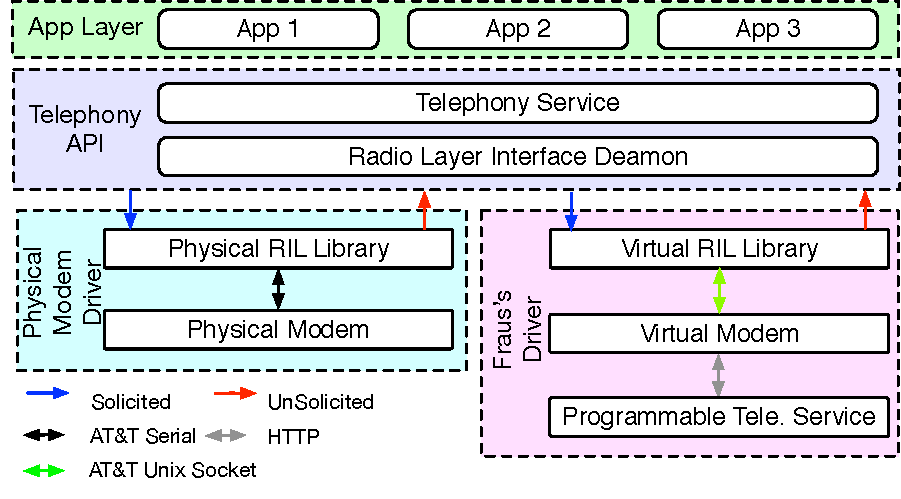
\includegraphics[width=0.43\textwidth]{Figures/rild}
	\caption{Overview of the Android Telephony Architecture}
	\label{fig:rild}
	\vspace{-0.4in}
	\end{center}
	\end{figure}

	% \subsection{How the Android Enable Wireless Communication} 
	% Android operating system is a stack of software components which is roughly divided into four main layers as shown below in the diagram. 

	% \textbf{Linux Kernel.} The foundation of the Android platform is the Linux kernel, which contains essential operating system functionalities such as threading and low-level memory management. It also includes the essential hardware drivers for WiFi and Bluetooth. 

	% \textbf{Hardware Abstraction Layer (HAL).} As the drivers interfaces provided by the kernel may vary from vendor to vendor. The Android system introduces a hardware abstraction layer (HAL). It provides standard interfaces that expose device hardware capabilities to the higher-level Android framework. For instance, the radio interface layer  daemon (RILD) offers a unified interface regardless of the radio hardware model. Fig demonstrates the workflow of RILD in a real device. It can be seen that the RILD act as a bridge between the cellular modem and the Android framework. On one hand, the RILD receives the commands (e.g., dial a phone number and hang up) originated by the Android framework and forwards them to underlying hardware. These commands are referred to as solicited commands.
	% On the other hand, the RILD also continuously monitors the responses of those commands and other phone events (e.g., call established and new message arrived) that originated from the underlying hardware. The responses and phone events are called unsolicited commands, of which RILD will notify the upper framework. Note that as an emulator does not equip with a cellular modem, the RILD simply remains asleep.

	% \textbf{Android Framework.} The Android framework is a set of system services that collectively form the environment in which Android applications run and are managed \cite{}.  Application developers are allowed to make use of these services in their applications. For instance, the telephony service is in charged of performing actions such as dialing a phone number or sending a text message. The WiFi service is managing all aspects of WiFi connectivity (e.g., scanning and joining networks). The activity manager controls all aspects of the lifecycle of every application.

	% \textbf{Applications} Located at the top of the Android architecture are a set of core applications such as phone dialing and messaging. The applications can provide key capabilities to third-party applications. For example, an application could simply invoke the messaging application to deliver a message to the recipient specified.

	% % \begin{figure}[ht]
	% % \begin{center}
	% % \includegraphics[width=0.42\textwidth]{Figures/Rild}
	% % \caption{Typical system deployment.}
	% % \label{fig:deploy}
	% % \end{center}
	% % \end{figure}
	% \subsection{Emulating A Cellular Modem}
	% Thus, to integrate an emulated modem, we have to implement a fully functional virtual modem and its corresponding  RIL library as shown in Fig.~\ref{fig:rild}. The library supports the necessary actions that allow the upper layer to send/receive messages and to query IMSI and IMEI. The requests are translated to AT\&T commands and sent to the virtual modem via a Unix local socket. The virtual modem is in essence a user space program and keeps handling the received commands. 

	% To send/receive a message, the virtual modem takes advantage of several online virtual number services such as Twilio and Nexmo. These services allow the virtual modem to acquire a mobile phone number programmatically via HTTP connections. The number then can be used to receive in-bound text messages. 



	 % after obtaining the phone number because we need some. Similarly, IMEI is randomly generated using the application. 

	% More specifically, as shown in Fig,  Fraus implements and registers an emulated cellular modem driver that RILD can talk with. The driver accepts the solicited commands (e.g., dial numbers and send messages) from the RILD. The commands will be translated into corresponding APIs provided by the virtual number services. Meanwhile, the driver periodically checks whether there is a new message. If so, it then generates an unsolicited commands and delivers it to the RILD. 

	% The whole process is transparent to the framework layer and application layer. From the applications' perspective, the emulator instance is now binding with a functional phone number and receiving a verification code.

	% \subsection{Emulating WiFi and Bluetooth}
	% \subsection{Implementing Virtual Wireless Interface}


	% is designed to run and test user space programs, especially, \textit{wpa\_supplicant} \cite{berg2009wifi}. The supplicant happens to be the most essential component in the Android WiFi system. Thus, without modifying any codes, the WiFi system could directly work on the simulated interface. 

	% Last obstacle to bypass the device profile authentication is the empty Device ID of emulators. For a physical device, the ID is randomly generated at the first time the user sets up the device and should remain constant. The ID then can be obtained through the \textit{Setting Provider} API. However, in an emulator, the API is hard-coded to return an empty value. To address this issue, we patch the \textit{Setting Provider} such that it can produce a random Device ID.

	%  However, we observe that an emulator simply retur
	% . However, we can observe
	% that “Device ID” is independently (and randomly) created
	% from an Android device itself. Therefore we can generate new
	% Device IDs for an Android device without any restrictions.
	% Thus no changes to the framework are required.

	% simulate arbitrary number of IEEE 802.11 radios for mac80211.
	% Though these APIs will become deprecated and only return a constant dummy value in versions later than Android 6.0, several workaround 


	% Fraus enables WiFi and Bluetooth emulation by installing virtual WiFi and Bluetooth drivers in the Linux kernel.  mac80211\_hwsim is a Linux kernel module that can be used to simulate arbitrary number of IEEE 802.11 radios for mac80211
	% Specifically, a kernel module named \textit{mac80211\_hwsim} is utilized to simulate a WiFi radio interface.
	% For future usage, Fraus also offers APIs than entitle users to specific some information for the virtual interfaces. 



	% \textbf{System Applications}
	% A system application is merely an application which is placed under /system/app folder in an Android device. They enable users to perform common tasks such as dialing, messaging and photo taking. The apps can also provide key capabilities to third-party applications. For example, an application could simply invoke the messaging application to deliver a message to the recipient specified. 

	% However, we notice that these apps consume a considerable amount of RAM even an user does not start and use them. We investigate this phenomenon and find that the apps tend to preload themselves to RAM along with the system booting process. It brings an advantage that the starting time of those apps can be reduced for a better user experience. However, since an emulator may seldom use the system apps, preloading them potentially leads to a huge waste of memory. 

	%  To avoid this issue, Fraus modifies the source codes of the system apps to prevent them from pre-fetching. Specifically, an Android app can enable pre-fetching by either registering a listener for the event \textit{BOOT\_COMPLETED} or setting the property \textit{android:persistent} in the manifest file to be true. Fraus disables all listeners for the boot event and removes the persistent property if existed.


	% The Android multimedia framework includes support for playing variety of common media types, so that you can easily integrate audio, video and images into your applications. You can play audio or video from media files stored in your application's resources (raw resources), from standalone files in the filesystem, or from a data stream arriving over a network connection, all using MediaPlayer APIs.

	% % Skia is an open source 2D graphics library which provides common APIs that work across a variety of hardware and software platforms. It serves as the graphics engine for Google Chrome and Chrome OS, Android, Mozilla Firefox and Firefox OS, and many other products.

	% processing support for multimedia applications with the help of Open Graphics Library named OpenGL ES [16]. OpenGL ES is a cross-platform graphics API that specifies a stan- dard interface for GPU and the Android applications could invoke the APIs to directly interact with the GPU.

	\section{Preparing for Large-Scale Attacks}\label{deploymentarch}
	To alleviate attackers' burden of manually setting up and managing emulator instances in a large-scale MCFA, 
	Fraus provides an emulator cluster management system. The system features a distributed architecture such that it can cope with scalability and fault-tolerance issues. Furthermore, it provides high-level APIs that present a logically centralized view and conceal the details of the underlying distributed protocols.
	% The architecture is designed to handle scale-out and fault-tolerance
	%  
	% Fraus provides a distributed architecture depicted in Fig.~\ref{fig:deploy} for scale-out and fault-tolerance deployment in various cloud platforms. 
	% It is considered challenging to deploy and manage a massive number of virtual devices due to the following three reasons.
	% First of all, it would be cumbersome and labor-consuming to install system images and specify automation tasks manually in every device. Second, to monitor and control the huge number of devices, it may be inappropriate to adopt a simple centralized architecture since it fails to cope with the scale-out and fault tolerance issue when the number of virtual devices increases. In other words, a more sophisticated distributed architecture is required. Last, as stated in Section, in order to bypass the device-id authentication, each device should be assigned a unique device-id profile, for instance, a tuple \textit{(account, phone number, IMSI...)}). Otherwise, an account may be logged in two different virtual machines and the abnormality may be detected by the application provider, leading to the account's blocking. As there are limited available profiles, how to assign them to different devices without duplication under distributed environment remains difficult. 

	\subsection{Enabling Scale-out and Fault Tolerance}
	One important feature of our architecture is its support for scale-out. 
	% Instead of relying on a single management node to control all the devices, 
	As shown in Fig~\ref{fig:deploy},
	Fraus incorporates multiple management nodes named \textit{Device Manager},
	each of which acts as the exclusive controller for a proportion of emulator instances. 
	More specifically, an individual device manager is solely in charge of assigning MCFA tasks to and collecting status information from the emulator instances it controls. 
	Such an architecture ensures the scalability by adding additional device managers to the cluster when the number of instances increases. 

	The distributed architecture is also designed to provide fault tolerance. The intuition is that the architecture allows multiple redundant manager instances waiting to take over in case a manager fails. By this mean, the failed manager's work could be immediately redistributed to another manager.
	In details, an emulator, upon creation, will establish multiple connections with available managers, but exactly one of which will be elected as the \textit{primary manager} by performing a consensus-based leader election \cite{lynch1996distributed}. From that moment on, the primary manager starts controlling the emulator and the other managers remain idle. When the primary manager fails, an election will be held again and a newly-elected manager will take over the emulator.


	Fraus implements the above mechanism with the help of Multicast DNS (mDNS) \cite{ververidis2008service} and ZooKeeper \cite{hunt2010zookeeper}. Specifically, mDNS enables an emulator to discover and connect to the IP addresses of available device managers.  ZooKeeper is utilized to perform leader election and failure detection. A manager must contact the ZooKeeper ensemble in order to become the primary manager for an emulator. If a manager loses its connection with ZooKeeper, a failure will be announced and another manager will attempt to take over the control by undergoing an election. 

	% Note that ZooKeeper maintains strong consistency among managers and remains fault tolerant so long as the majority of managers are available.


	% One key feature is that 
	\subsection{Presenting a Logically Centralized View}
	% To cope with these challenging issues, Fraus provides a distributed device management architecture as depicted in Fig~\ref{fig:deploy}. This architecture features a transparent view for users by providing a set of high-level APIs hiding the underlying details. 
	% In other words, an user can easily program and deploy an automation task without concerning how the virtual devices are set up or how the tasks are actually carried out in each device under distributed environment. 

	% Our architecture offers a high-level API abstraction. It allows an us


	% Fraus aims to provide a high-level API abstraction. It allows an user to easily program and deploy automated  attacks without concerning how the emulators are set up or how the tasks are delivered to each emulator under the distributed environment.
	Although the cluster is now running across  multiple device managers, Fraus preserves the simplicity of a centralized architecture with a useful API abstraction exposing a logically centralized view. It allows individuals to program and launch attack tasks without concerning the low-level details such as how the emulator instances are set up and how the tasks are dispatched and executed under the distributed environment.

	Specifically, Fraus provides four types of APIs which cover every aspect of a large-scale MCFA:
	\begin{enumerate}
	\item{Development APIs.} Deployment APIs allow users to specific the number of emulators needed in each MCFA.
	\item{Automation APIs.} Automation APIs assist individuals to compose the GUI automation scripts for an application.
	\item{Configuration APIs.} Configuration APIs entitle users to adjust the setting of an emulator (e.g., device profile and network configuration).
	\item{Monitor APIs.} Monitor APIs provide real-time information of each emulator (e.g., memory or CPU usage).
	\end{enumerate}

	Figure~\ref{fig:deploy} depicts the implementation details of these APIs. They are implemented on top of a set of open-source building blocks. Specifically,
	The deployment APIs rely on \textit{Vagrant} \cite{hashimoto2013vagrant} for creating and maintaining virtual machine instances in physical servers. We also extend the original Vagrant with a variety of plug-ins to bring the support for various cloud platforms. 

	The automation APIs encapsulate an Android testing framework named \textit{Cucumber} \cite{kulkarni2016deployment}. It enables users to express the automation instructions using natural language that can be easily understood by non-technical individuals. For instance, an user can easily enter his username to an application with a simple instruction like \textit{Enter text `username' into field with id `username\_textfield'}. Note that if the user is not in favor of the automation APIs, he can also choose other automation frameworks written in a variety of languages such as Python and Ruby. 

	The configuration APIs and monitor APIs make use of the distributed database \textit{Cassandra} \cite{lakshman2010cassandra} to maintain the configuration and status information of every emulator. In details, Cassandra serves as a hub facilitating information exchange between users and emulators. For instance, the status information from an emulator is stored in the database and can be queried by users in the near future. Similarly,
	configurations specified by users are stored in the database and they can be retrieved by emulators via polling.

	Note that the above building blocks run in each device manager. Each manager can synchronize its information with others using ZooKeeper and Cassandra such that everyone has the access to the global information to provide the logically centralized view. 


	% One challenging issue lies in the implementation of the configuration APIs. 
	% The API requests will be operated on top of the data stores and later propagated to the devices. 
	% Note that Cassandra can handle large amounts of data and maintain eventual consistency, while Zookeeper provides strong consistency but less storage volume. The two datastores complement each other and greatly facilitate the system implementation.

	% One challenging issue lies in how to automatically assign device profiles to various emulator instances without duplication. We achieve this by utilizing the combination of Cassandra and Zookeeper. Specifically, we assign each available device profile with a unique identifier and store them in Cassandra. Upon creation of every emulator, its primary manager will inquire the ZooKeeper ensemble for a unique identifier of an unoccupied device profile. After getting the identifier, the manager can query the Cassandra for the corresponding device profile. Besides, the manager will periodically send heartbeat signals to the emulators it controls. Once a device is not responding (i.e., not longer alive), the manager will reclaim its profile and assign it to another emulators. 
	% Owning to the strong consistency level of ZooKeeper, it can be guaranteed that no duplicated device profile identifier will be issued. Thus no duplicated device profile will be assigned. Meanwhile, the eventual consistency level of Cassandra can ensure the availability of profiles in every manager instance nearly all the time. 


	% Note that Cassandra and Zookeeper maintain eventual consistency and strong consistency respectively, thus Cassandra will be mainly used to store 
	\begin{figure}[tb]
	\begin{center}
	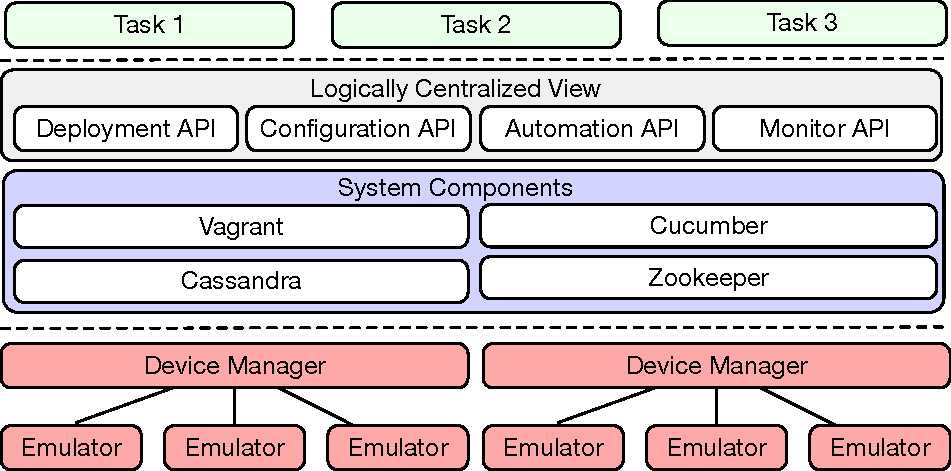
\includegraphics[width=0.44\textwidth]{Figures/networkarchitecture}
	\caption{System Architecture.}
	\label{fig:deploy}
	\vspace{-0.3in}
	\end{center}
	\end{figure}


	% 









	\section{Experiments}\label{expm}
	In this section, we provide detailed evaluation on Fraus in terms of application compatibility, resource savings, and cluster deployment. 


	\subsection{Ethical Considerations}
	Note that the main motivation is to raise public awareness of the effectiveness and simplicity of launching a MCFA using Fraus. Therefore, all the following experiments are carefully designed such that they incur neither monetary damages nor service interruptions.



	\subsection{Application Compatibility} 
	To evaluate the the application compatibility, we implement an automation script that downloads and runs the top 300 applications from the Google Play Store on Fraus. Note that a large partition of them are games, which are the hardest applications to support because of their CPU-intensive and graphics-intensive nature. For comparison purposes, the experiment is carried out in the Android official emulator. 

	The experimental results show that 96\% of the applications run successfully on Fraus, while in the Android official emulator only 59\% can start properly. Fraus is highly stable and compatible with existing applications. Out of curiosity, we also pinpoint the causes of the failed cases.
	We discover that the official emulator failed to run most programs mainly because of the device profile scrutiny and the buggy GPU emulation, which frequently leads to the crash of the graphics system. These problems do not affect Fraus, which only fails to run a small number of applications due to CPU emulation defects. In brief, certain uncommon CPU instructions used by the applications are not properly emulated, leading to the crashing situations. The defects allow us to tell Fraus apart from physical devices, which can be used as a countermeasure to combat Fraus. We will discuss it in details in Section~\ref{countermeasure}.


	 % and realize that it is mainly attributed to the CPU emulation defects. This motivates us the countermeasures to combat Fraus, which will be demonstrated in Section~\ref{countermeasure}.
	% To investigate how many applications our Fraus system can support, we install 30 popular social-media and advertisement applications, which are the common victims of the click fraud. Most of the applications involve complicated system functionalities such as video playback and SMS delivery. Thus, they are supposed to be the hardest applications to support. Our system is able to run all the 30 applications as normal, which demonstrates that our system has a very good application coverage and fair stability.

	\subsection{Resource Savings}
	To measure the CPU saving of Fraus, we select 6 popular social-media and advertising applications including \textit{Facebook}, \textit{Wechat}, \textit{Instagram}, \textit{Tumblr}, \textit{DailyCash} and \textit{LuckyCash}, which are the frequent victims of the MCFA. Specifically, every application is automated to perform predefined tasks such as clicking a like button or viewing a video clip. Each task is performed for 30 times and the average CPU usage is reported. Note that 
	the CPU usage retrieved from the \textit{top} command in Android only updates every one second, which is relatively coarse-grained. We overcome the issue by directly polling the contents from the system file \textit{/proc/stat}, which provides the almost real-time CPU usage. For comparison purposes, we repeat the experiments on the official emulator.

	Figure~\ref{fig:cpusaving} demonstrates the experimental results. It can be seen that 
	Fraus significantly suppresses the CPU utilization. For instance, Wechat consumes approximately half of the CPU resource on the unoptimized official emulator, while Fraus manage to decrease the workload to 14.7\%. A more obvious example is that LuckyCash on the official emulator nearly exhausts the CPU, while the same application on Fraus only incurs tiny CPU usage of 17.9\%, which is an approximate 90\% reduction. A closer look at the usage of each system process reveals that the saving is mainly attributed to the Surfaceflinger and Mediaserver processes. It is expected as their core computation is evaded in Fraus.

	 
	We also obtain the memory statistics of Fraus with the help of the \textit{ps} command. The footprint of Fraus is approximately 190 MB, which is significantly smaller than the official emulator that nearly consumes 500 MB. The 60\% memory reduction indicates the effectiveness of the lazy loading mechanism. 
	% Besides, the social media applications appear to benefit more from the optimized Surfaceflinger process. It is mainly due to the applications typically have complicated GUIs, which pose heave burden on the Surface Flinger. On the other hand, the advertisement applications harvest more CPU power from the Media Server process because they need to play video clips frequently.


	\begin{figure}[tb]
	\begin{center}
	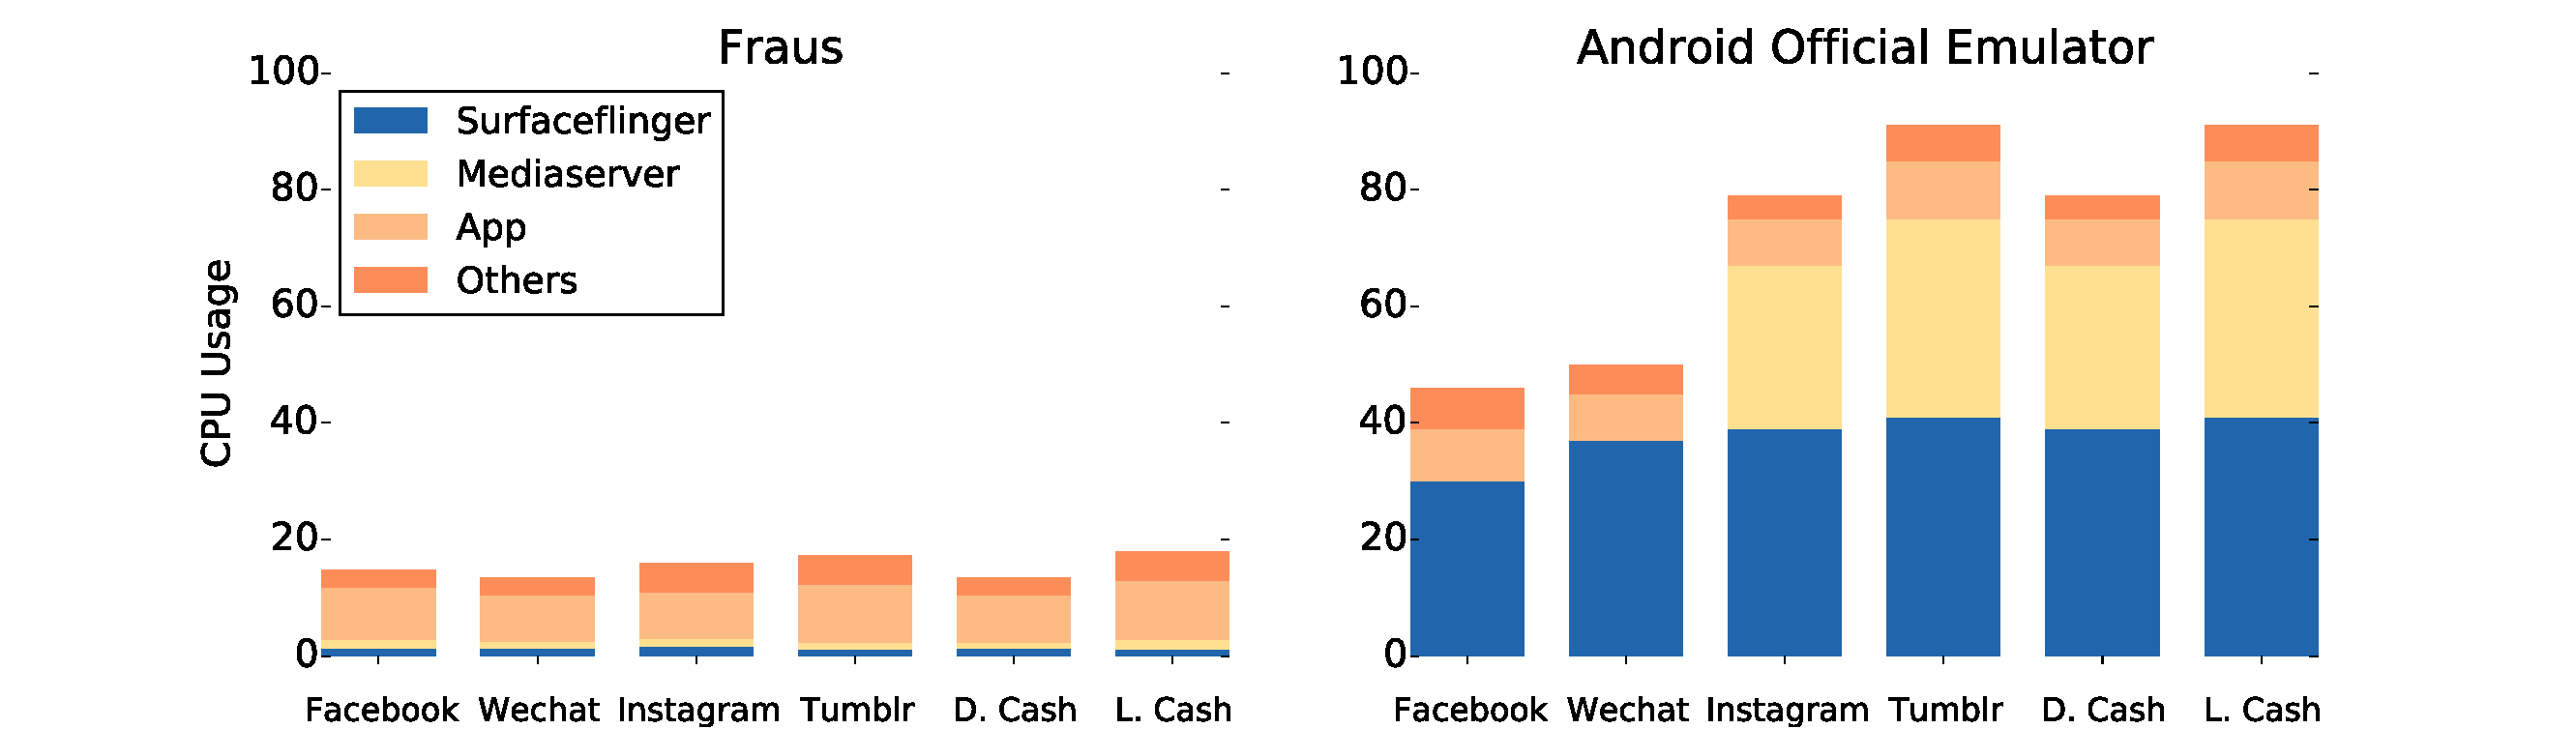
\includegraphics[width=0.48\textwidth]{Figures/cpusaving}
	\caption{Histogram of Elapsed Time for Three Devices}
	\label{fig:cpusaving}
	\vspace{-0.3in}
	\end{center}
	\end{figure}





	%The savings are mainly attributed to that Fraus bypasses the compute-intensive display functionality, which is originally carried out by the Surface Flinger and Media Server.
	% \begin{table}[]
	% \centering
	% \caption{CPU usage for the selected applications in the Official Android Emulator and Fraus}
	% \label{my-label}
	% \begin{tabular}{|p{1.2cm}|p{1.2cm}|p{0.7cm}|p{0.7cm}|p{0.5cm}|p{0.6cm}|p{0.8cm}|}
	% \hline
	% \multicolumn{2}{|p{0.5cm}|}{App. Name}   & S.F. & M.S. & App. & Others & Total \\ 
	% \hline
	% \multirow{2}*{Wechat}  &Official  & 37.1\% & 0\% & 9.3\% & 6.1\% & 52.5 \%  \\
	%        & Fraus & 2.1\% & 0\%  & 8.2\% & 5.0\% & 15.3\% \\
	% \hline   

	% \multirow{2}*{Facebook}  &Official  & 46.2\% & 0\% & 4.2\% & 9.1\% & 52.5 \%  \\
	%        & Fraus & 1.1\% & 0\%  & 4.3\% & 8.9\% & 14.3\% \\
	% \hline  

	% \multirow{2}*{Twitter}  &Official  & 37.1\% & 0\% & 9.3\% & 6.1\% & 52.5 \%  \\
	%        & Fraus & 2.1\% & 0\%  & 8.2\% & 5.0\% & 15.3\% \\
	% \hline  

	% \multirow{2}*{Tumblr}  &Official  & 37.1\% & 0\% & 9.3\% & 6.1\% & 52.5 \%  \\
	%        & Fraus & 2.1\% & 0\%  & 8.2\% & 5.0\% & 15.3\% \\
	% \hline  

	% \multirow{2}*{Instagram}  &Official  & 37.1\% & 0\% & 9.3\% & 6.1\% & 52.5 \%  \\
	%        & Fraus & 2.1\% & 0\%  & 8.2\% & 5.0\% & 15.3\% \\
	% \hline  

	% \multirow{2}*{LuckyCash}  &Official  & 37.1\% & 98\% & 9.3\% & 6.1\% & 100 \%  \\
	%        & Fraus & 2.1\% & 1.5\%  & 8.2\% & 5.0\% & 15.3\% \\
	% \hline  

	% \multirow{2}*{DailyCash}  &Official  & 37.1\% & 100\% & 9.3\% & 6.1\% & 100 \%  \\
	%        & Fraus & 2.1\% & 1.3\%  & 8.2\% & 5.0\% & 15.3\% \\
	% \hline  

	% \multirow{2}*{MoneyRain}  &Official  & 37.1\% & 67\% & 9.3\% & 6.1\% & 100 \%  \\
	%        & Fraus & 2.1\% & 1.6\%  & 8.2\% & 5.0\% & 15.3\% \\
	% \hline  

	% \multirow{2}*{WatchEarn}  &Official  & 37.1\% & 78\% & 9.3\% & 6.1\% & 100 \%  \\
	%        & Fraus & 2.1\% & 1.7\%  & 8.2\% & 5.0\% & 15.3\% \\
	% \hline  

	% \multirow{2}*{Light}  &Official  & 37.1\% & 89.1\% & 9.3\% & 6.1\% & 100 \%  \\
	%        & Fraus & 2.1\% & 2.1\%  & 8.2\% & 5.0\% & 15.3\% \\
	% \hline  


	% \end{tabular}
	% \end{table}
	\subsection{Cluster Deployment}
	We launch a large-scale mocking attack with the help of the Fraus' cluster management system. Specifically, we set up a cluster running across four physical servers (Intel i7-6700 3.40 GHz CPU and 32GB RAM). The servers utilize the \textit{KVM} hypervisor to provide virtual machine containers. 
	We allocate each container with 512 MB RAM and one virtual CPU. Theoretically, a physical server then can hold less then 64 instances simultaneously. In reality, owning to the small resource demand of Fraus, we manage to fit 125 instances, indicating the high cost efficiency. 
	% Meanwhile, the CPU seems not be a bottlecneck for the cluster
	% Nevertheless, the reality thanks to the KSM deduplication technique, we manage to fit 125 instances in each physical server. 
	Inevitably the huge number of instances may push the server's CPUs to its limit. Nevertheless, the impact is limited because most Android applications are not time-critical and can bear the small delay caused by the insufficient CPU power.


	% We evaluate our prototype system in terms of the application coverage, memory and CPU usage and system overhead.

	\section{CounterMeasures}\label{countermeasure}
	% Fraus significantly reduces the cost to launch a large-scale MCFA by taking advantages of device emulators. 
	In this section, we propose two feasible countermeasures to combat Fraus. 
	% The countermeasures can be combined with any existing approaches to further enhance the resistance. 
	The intuition underlying our countermeasures is that applications can detect the emulator environment and refuse to perform any activities by terminating or stalling the execution. The most common approach to detect
	the presence of an emulator environment is based on the fingerprinting of the runtime environment. This includes checking for specific artifacts, such as some specific environment variables, background processes, or defective results obtained from certain API interfaces \cite{vidas2014evading}. However, we argue that these methods are not fully reliable because an attacker can always modify the system source codes to build a deceiving runtime environment.

	Instead, our approaches detect the Fraus environment by checking the platform-specific characteristics that are different with respect to a physical device.
	The characteristics include a tiny defect in the CPU instruction set and significantly different timing properties of the graphics system.

	\textbf{Examining CPU Instruction Sets.}
	% To understand the approach, we have to briefly elaborate some virtualization knowledge. 
	An emulator is typically X86-based in pursuit of performance, because the readily-available X86 instructions can be directly executed owning to the Hardware Virtualization technology.
	Nevertheless, the X86-based emulator has to handle a practical issue; because nearly all physical devices are equipped with ARM CPUs, various Android applications written in C/C++ are solely compiled with the ARM instruction set, which cannot be directly executed by X86-based system. To address this issue, a binary translator named \textit{native bridge} is utilized to translate the instructions from ARM to X86. 

	% Thus the applications cannot be directly run in a X86-based system. To address this issue, the X86-based system adopts 
	Our first approach makes use of the fact that the binary translator does not provide support for the ARM \textit{NEON} CPU instruction set, which is intended for accelerating audio and video encoding. This defect offers us a chance to distinguish whether the device has an ARM CPU. In details, an application can embed a C program containing the ARM NEON instructions. If the program can be successfully loaded, it means the device is equipping with an ARM CPU and it is not likely an emulator. 

	% could be obtained by compiling the Android source codes using  compiler toolchains for different CPU architectures (e.g., ARM and X86). The ARM-based image and X86-based image will have a huge performance difference because the virtual machine has to handle them quite differently. When running the ARM-based image, the virtual machine utilizes a technique named \textit{Binary Translation} to continuously translate sequences of ARM instructions to X86 instructions. The X86 instructions then can be executed by the virtual machine which is hosted in a physical machine equipped with X86 CPUs. The translation process is generally considered slow and inefficient. On the other hand, when running a X86-based image, the virtual machine can directly execute the readily-available X86 instructions owning to the \textit{Hardware Virtualization}, which significantly reduces the virtualization overhead. Therefore, nearly all emulators use the X86-based image in pursuit of performance. Nevertheless, the X86-based system still has to handle a practical issue; a great number of C/C++ based applications only compile the source code to ARM instructions. Thus the applications cannot be directly run in a X86-based system. To address this issue, the X86-based system adopts a binary translator named \textit{native bridge} to translate the applications' ARM instructions. 

	\begin{figure}[t]
	\begin{center}
	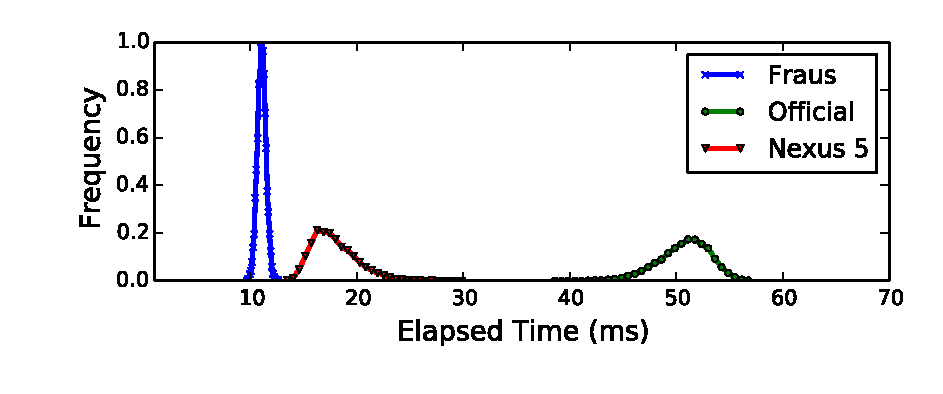
\includegraphics[width=0.44\textwidth]{Figures/elapse}
	\caption{Normalized Histogram of Elapsed Time for Three Devices}
	\label{fig:elapse}
	\vspace{-0.4in}
	\end{center}
	\end{figure}

	\textbf{Examining Timing Properties of the Graphics System.} 
	Fraus evades the intensive graphical computation in order to save CPU processing power. However, it comes with a side effect that the timing properties of the graphics system are affected. For instance, the time consumed by an application to draw a frame is significantly shortened.
	 To demonstrate the effect, we first implement a test program that renders a rotating 3D color-cube and measures the elapsed time per invocation of the draw() method (i.e., time consumed to draw a frame). The program is then tested on two emulators including the official emulator and Fraus as well as a physical device LG Nexus 5. For each device, we sample the elapsed time for 10000 frames and report the histogram in Fig.~\ref{fig:elapse}.

	One important finding is that the devices are statistically different from each other (Wilcoxon, $p \le 0.001$). For example, Fraus and Nexus 5 possess a median of 11 ms and 18 ms respectively, while the statistics value for the official emulator soars into 59 ms. Thus, we can easily rule out the official emulator. Meanwhile, we notice that Fraus exhibits a bell curve with observable measurements from 9 to 11 and the majority of measurements are clustered closely around the median. In contrast, Nexus 5 presents a right skewed distribution ranging from 12 to 27 with the data points spreading far from the median. The difference are mainly due to that in a physical device, the elapsed time likely varies depending on the complexity of each frame. For instance, it consumes more time to draw a frame filling with 10 triangles than those only with 1 triangle. Conversely, the complexity does not affect Fraus because the involved computation is skipped and the elapsed time for each frame should remain highly consistent. 

	% Meanwhile, the GPU in a physical device tends to reduce its performance to cope with the overheating issue, leading to the right-skew distribution.

	Based on the above observations, heuristics can be devised to detect the Fraus runtime environment. Specifically,
	We first measure the standard deviation $s$ of the sample. After that, we  obtain the L-skewness statistics $r$ \cite{joanes1998comparing} as follows:
	\begin{equation}
	r = \frac{\frac{1}{3}\binom{n}{3}^{-1}\sum_{i=1}^{n}\left \{ \binom{i-1}{2} - 2\binom{i-1}{1}\binom{n-i}{1} + \binom{n-i}{2} \right \}x_i}
	{\frac{1}{2}\binom{n}{2}^{-1}\sum_{i=1}^{n}\left \{ \binom{i-1}{1} - \binom{n-i}{1} \right \}x_i},
	\end{equation}
	where $x_i$ represents the $i$th sample. We will claim Fraus is detected if $s \le 1$ and $abs(r) \le 0.05$. The intuition behind the
	heuristic is that a tiny $r$ and $s$ indicates a highly-symmetry and tightly-coupled bell curve, which is the Fraus's unique feature. 
	% Nowadays, GPUs tend to create abundant heat energy when they are heavily utilized. To prevent overheating, mobile devce systems have to reduce the GPU’s operating frequency and suppress its performance when its temperature exceeds certain thresholds. 


	% Fraus and Nexus 5 exhibit a significantly lower elapsed time than the official emulator. In details, Fraus and Nexus 5 possess a median of 11 ms and 18 ms respectively, while the statistics value for the official emulator soars into 59 ms. This phenomenon is expected because Fraus simply skips the graphical computation while Nexus 5 efficiently conducts the computation on a GPU. 

	% The observation that really benefits us is that Fraus exhibits a bell curve with observable measurements from 8 to 13, while Nexus 5 presents a right skewed distribution ranging from 12 to 27. By taking a closer look, we will find that Fraus is more stable because the majority of measurements of Fraus are clustered closely around the mean. In contrast, the data points for Nexus 5 spread far from the mean. The performance instability may be due to the overheating issue of GPUs. Nowadays, GPUs tend to create abundant heat energy when they are heavily utilized. To prevent overheating, mobile device systems have to reduce the GPU’s operating frequency and suppress its performance when its temperature exceeds certain thresholds. 

	% From the experimental data, heuristics can be devised to detect Fraus. In details, we can measure the Fisher-Pearson coefficient of skewness and kurtosis for the two distributions. The skewness $G_1$ can be expressed as 

	% \begin{equation}
	% G_1 = \sum_{1}^{N}(y_{i} - \mu)/ (N \times s^3)
	% \end{equation}
	% \begin{equation}
	% % \sum_{1}^{N}(y_{i} - \mu)/ (N \times s^3)
	% % (N \times s^3)

	% \end{equation}





	% The second approach is far more difficult to be circumvented. When running a C/C++ application with the help of binary translator, an ARM instruction may be translated into a certain number of X86 instructions for execution. The number is mainly decided by the translator and varies from instruction to instruction. 

	% We observe that a C/C++ based application is at a natural disadvantage when it comes to processing speed because An ARM instruction may have to be translated into multiple X86 instructions for execution. The observation has been documented in the research work \cite{vidas2014evading} where a C program calculating the first 1,048,576 digits of Pi is executed on an emulator and physical devices respectively. The execution time in the emulator will be significantly longer than the physical devices. Therefore, the execution time could be an affective statistic for emulation detection by adapting Wilcoxon test.

	% the viability of the this emulation detection technique.

	% However, the absolute execution time may not be an accurate statistic for emulation detection because the new-generation devices also consumes much less execution time compared with the old-generation ones. To reduce the effect of the performance gap between physical devices, we create another reference program conducting basic mathematical calculations (e.g., 1 million times of multiplications). Then we can obtain the execution time ratio between the PI-calculation and reference program. The execution time ratios of physical devices remain close due to the similar CPU architectures but vary significantly from the execution ratio of an emulator.

	% However, this method does not consider the performance difference among various CPU
	% In this paper, we improve this detection method in two aspects. First of all, 

	% instead of relying on the absolute execution time, we change 

	%  of Pi using the method illustrated in \cite{ooura1999improvement}. The calculation is considered CPU-intensive as it requires extensive use of Fast Fourier Transforms, square roots and multiplication. The program is compiled into ARM instructions and runs on the emulator and two physical devices including Nexus 5 and Nexus 6P. Every execution takes averagely 48.7 seconds, 12.3 seconds, and 9.4 seconds on the emulator, Nexus 5 and Nexus 6P respectively.


	% We instead turn to a crude method of benchmarking: evaluating
	% the duration of lengthy computations. We created a Java Native
	% Interface (JNI) application for Android using the NDK. Our application
	% calculates the first 1,048,576 digits of Pi using the method
	% described by Ooura [29]. Pi is calculated over 16 rounds of increasing
	% precision using Arithmetic-Geometric Mean (AGM) making
	% extensive use of Fast Fourier Transforms, square roots, multiplication,
	% etc.
	% The AGM calculation shows significantly different results when
	% comparing emulated instances with similar physical devices. Table
	% 4 shows the average and standard deviation for several tested
	% devices. For instance, executing the native application on a 4.2.2
	% emulator results in an median round duration of 68.8 seconds with
	% a total execution time of 1101.9 seconds. A 4.2.2 Galaxy Nexus
	% demonstrates a 16.8 second median round duration, and takes 268.8
	% seconds to complete. Comparatively, the PC hosting the emulator
	% executes the same code 2.5 seconds with a median of 0.15 second/round
	% (Linux PC). Round durations show statistically signifi-
	% cant differences between emulated and non-emulated environments
	% (Wilcoxon test, W = 256, p < .001), which in turn demonstrates
	% the viability of the this emulation detection technique.


	% Specifically, Android supports apps written either in Java or C/C++ languages. Regarding the apps purely written in Java, the underlying CPU architecture is transparent to them as the Java compiler has transformed their source codes to platform-independent byte codes. As for the apps with components written in C/C++, the Apps are likely to crash because the C/C++ components have been compiled to ARM instructions, which are incompatible with X86 platforms. Though a small number of apps are shipped with x86 versions, the other apps will not be able to run in the emulator.
	 % aFraus compile the Android system from source for x86 platforms. By doing this, the emulator can avoid the excessive overhead of ARM instruction emulation. 

	% Despite that the idea is straightforward, practically implementing it entails a challenging issue. Specifically, Android supports apps written either in Java or C/C++ languages. Regarding the apps purely written in Java, the underlying CPU architecture is transparent to them as the Java compiler has transformed their source codes to platform-independent byte codes. As for the apps with components written in C/C++, the apps are likely to crash because the C/C++ components have been compiled to ARM instructions, which are incompatible with x86 platforms. Though a small number of apps are shipped with x86 versions, the other apps will not be able to run in the emulator.

	% To address this issue, Fraus adopt a technique introduced in []. The technique allows real-time binary instruction translation from ARM to x86. Note that compared with the official Android emulator, our approach merely translates a small number of components with ARM instructions such that a great amount of overhead is avoided.

	\section{Related Work}\label{related}
	% \textbf{Marware-based Attacks}

	MCFA is a serious threat to the Internet economy. From an economics viewpoint, the research work \cite{kshetri2010economics} investigates the mechanisms and processes associated
	with the click-fraud industry. Miller et al. \cite{miller2011s}, on the other hand, provides a detailed survey on the click fraud techniques. Specifically, there exists two common approaches to launch a MCFA. One is through mobile malware \cite {felt2011survey}, which performs click actions stealthily as a background task. MadFraud \cite{crussell2014madfraud} further discovers that the click fraud malware attempts to
	remain stealthy by only periodically sending clicks. Nevertheless, the power of this attack is of uncertainty because it is mainly decided by the number of infected phones. Moreover, the advance of security countermeasures such as \cite{liu2015efficient} and \cite{nath2015madscope} also renders a majority of click fraud malware ineffective. Thus, attackers shift their focus on the second method, referred to as `click farms' \cite{juels2007combating}. A typical click farm deploys thousands of mobile devices and automates them to generate click events by computers. Clearly, the power of this approach is increased along with the number of devices, however, which also incurs a substantial purchasing expense. One alternative to the expensive physical devices is emulators.
	Though emulators have been utilized in a great amount of literature for runtime analysis \cite{arzt2014flowdroid} and malware detection \cite{yan2012droidscope}, little research has been conducted to investigate the usability of emulators on MCFA. We bridge the gap by presenting Fraus, that enables us to launch a MCFA with emulators.

	To prevent the MCFA, a number of countermeasures have been introduced. The simplest solution is to use threshold-based detection; 
	if a huge number of click events with the same device profile are received, they can be considered as fraud. This approach is not effective as device profiles can be easily modified. More sophisticated solutions are typically based on data-mining techniques \cite{zhu2017ad}. For example, the research work \cite{zhang2008detecting} utilizes group Bloom filters over click event time series to detect the fraud. Another interesting approach is to use bait contents \cite{haddadi2010fighting} to check whether clients are automated.
	We can combine these approaches with our proposed countermeasures to further increase the resistance against Fraus.
	% Although a number of countermeasures such as \cite{cho2016combating} and \cite{zhu2017ad} have been proposed over the past years, most application providers are reluctant to deploy them due to the economy inefficiency \cite{cho2016combating}. 

	% \section{Discussion}\label{discussion}
	% Fraus has enabled launching cost-efficient and scalable click fraud attack via Android emulators. Still, it bears several limitations that needs further improvement.

	% \textbf{Low Monitoring Performance and Visibility}
	% In the distributed management system, the monitoring APIs are implemented using the polling approach. In other words, some tasks may have to poll the database periodically to detect changes in virtual devices' states. This inevitably increases the CPU load while simultaneously aggravated the delay for reacting to status information. To address these issues, we plan to integrate event notification mechanism with the help of distributed message broker \textbf{RabbitMQ}. Meanwhile, we begin putting our focus on improving the speed of database operations by incorporating the low latency distributed key-value
	% store \textbf{RAMCloud}.


	\section{Conclusion}\label{conclusion}
	In this paper, we raise public concerns of the simplicity of launching a large-scale MCFA by presenting Fraus. Fraus has a tiny CPU and memory resource demand. Besides, Fraus can generate a seemingly authentic device profile and disguise itself as a legitimate device. To facilitate a large-scale attack, Fraus also provides a distributed emulator cluster management system, which is scalable and fault-tolerant. We evaluate the performance of Fraus and demonstrate that Fraus has high application compatibility and cost efficiency. Finally, we also propose countermeasures leveraging Fraus's platform-specific characteristics to combat such an attack.

	\begin{spacing}{0.8} 

	\bibliographystyle{IEEEtran}
	\bibliography{myrefs}
	\end{spacing}
	\end{document}

